% Prova 01 remediation --- Q2 topics: Solow golden rule, two-period household, competitive equilibrium and its law of motion.
% Error clusters 2-4 of Prova/prova-01-error-analysis.md. Book exercises are reproduced verbatim with a source line (user request).
% \solucoesfalse -> blank list ; \solucoestrue -> answer key + rubric.
% Compile from this folder: pdflatex (2x, per-job jobname, see .agent/notes/latex-lists-build.md); pdffonts (all Type 1).
% Every symbolic and numeric result: practice-P1-growth-ge-check.py
\documentclass[11pt,a4paper]{article}
% Shared preamble of the practice lists (practice-L*.tex), adapted from lista-exam.tex.
% Each list sets \solucoesfalse / \solucoestrue and \listatema right after \input{practice-preamble}.
\usepackage[utf8]{inputenc}
\usepackage[T1]{fontenc}
\usepackage{lmodern}   % Type 1 vector fonts (replaces PK bitmaps)
\usepackage{cmap}      % ToUnicode CMap -> copyable text and accents
\usepackage[english]{babel}
\usepackage{amsmath,amssymb,amsfonts}
\usepackage[a4paper,margin=2.2cm]{geometry}
\usepackage{enumitem}
\usepackage{fancyhdr}
\usepackage{comment}
% One cut file per job, so builds running side by side cannot swap each other's solutions.
\def\DefaultCutFileName{\def\CommentCutFile{\jobname.cut}}
\usepackage{xcolor}
\usepackage{microtype}
\usepackage{booktabs}
\usepackage{tikz}
\usepackage{pgfplots}
\pgfplotsset{compat=1.16}

\newif\ifsolucoes
\newcommand{\disciplina}{Macroeconomics I --- MPE Insper}
\newcommand{\espacoresol}{4.5cm}   % height of the answer space in the blank list
% The sol environment must be decided after the list sets its toggle.
\AtBeginDocument{\ifsolucoes\includecomment{sol}\else\excludecomment{sol}\fi}

\pagestyle{fancy}\fancyhf{}
\lhead{\footnotesize\disciplina}
\rhead{\footnotesize Practice list\ifsolucoes{} --- Solutions and rubric\fi}
\cfoot{\footnotesize\thepage}
\renewcommand{\headrulewidth}{0.3pt}
\setlength{\headheight}{14pt}
\setlist{topsep=2pt,itemsep=2pt}
\newcounter{questao}

\newcommand{\bloco}[3]{\par\bigskip\noindent
  {\large\bfseries\color{blue!55!black}Block #1 --- #2}\par\noindent\hfill\textit{(#3)}\par
  \noindent\rule{\linewidth}{0.3pt}\smallskip}
\newcommand{\questao}[1]{\par\refstepcounter{questao}\medskip\noindent
  \textbf{Question \thequestao.}~#1\par}
\newenvironment{alternativas}{\begin{enumerate}[label=\Alph*.,leftmargin=2.2em,topsep=1pt]}{\end{enumerate}}
\newcommand{\gabarito}[1]{\ifsolucoes\par\noindent\textbf{Answer:}~#1\fi}
\newcommand{\resolespaco}{\ifsolucoes\else\par\textit{Solution:}\vspace{\espacoresol}\par\fi}
\newcommand{\passo}[2]{\par\smallskip\noindent\textbf{Step --- #1.}~#2}
\newcommand{\intuicao}[1]{\par\smallskip\noindent\textit{Economic intuition.}~#1}
\newcommand{\refbib}[1]{\par\smallskip\noindent{\footnotesize\color{black!60}\textbf{Ref:} #1}}
\newcommand{\rubrica}[1]{\par\smallskip\noindent\textbf{Grading rubric.}\begin{itemize}[leftmargin=1.4em,topsep=1pt]#1\end{itemize}}

\newcommand{\cabecalho}{%
\begin{center}
  {\Large\bfseries \disciplina}\\[2pt]
  {\large Practice list: \listatema}\ifsolucoes\\[2pt]\textit{Solutions and grading rubric}\fi
\end{center}
\vspace{2pt}
{\footnotesize\noindent\textbf{Instructions.} Multiple choice: mark the single correct option (no
penalty for wrong answers). \emph{True/False}: every 2 wrong items cancel 1 right one
(score $=\max\{0,\text{right}-\text{wrong}/2\}\times$ item value); blank items do not count.
Discursive questions: show every step. Parameters are symbols with the stated admissible
ranges; answers are closed forms, conditions, signs and limits.\par}}

\newenvironment{notacao}{\par\smallskip\noindent\textbf{Notation.}\begin{itemize}[leftmargin=1.4em,topsep=1pt,itemsep=0pt]\small}{\end{itemize}}
\allowdisplaybreaks
\solucoesfalse                % <<<< \solucoestrue for the ANSWER KEY
\newcommand{\listatema}{Golden rule and the two-period competitive equilibrium (Prova 01, Q2)}
\renewcommand{\espacoresol}{5.5cm}
\setlength{\emergencystretch}{3em}   % lets the long \texttt paths in the Ref lines break cleanly

\begin{document}
\cabecalho

{\footnotesize\noindent\textbf{Notation (Kurlat 2020).} Capital share $\alpha$ in $Y=AK^\alpha L^{1-\alpha}$ (the exam wrote it
$\sigma$); $\sigma$ is reserved for the curvature of $u(c)=\frac{c^{1-\sigma}}{1-\sigma}$ ($1/\sigma$ is the intertemporal elasticity of substitution,
$\sigma=1$ is $\ln c$); $\beta\in(0,1)$ discount factor, $\rho\equiv1/\beta-1$; $\delta$ depreciation; $n$ population growth; $a$ assets
carried into the next period; $r^K$ rental rate of capital, $r$ interest rate, with $1+r=r^K+1-\delta$ (Kurlat (9.3.11)).
Lower-case $k$, $y$, $c$ are per worker unless stated. Book exercises are reproduced verbatim, in the book's own notation, after a source line; parts this list adds are marked.
\par
\noindent\textbf{What this list repairs.} (i) Golden-rule algebra: carry the exponent $\frac{\alpha}{1-\alpha}$, cross-check with
MPK $=n+\delta$, test a knife edge. (ii) The household problem: every choice variable and every income source, corners included.
(iii) Market clearing turns one household's saving rule into a law of motion $k_{t+1}=\phi(k_t)$; the saving rate it implies is
chosen, and need not be the golden-rule rate.\par}

% =============================================================================
\bloco{1}{Exam level: the golden rule and the two-period household}{Kurlat \S\S4.3, 6.2; Jones ch.~5 \,\textbullet\, 35 points}

\questao{(8 points) \textit{Source: Kurlat, P. (2020), \emph{A Course in Modern Macroeconomics}, Exercise 5.8 ``National Accounts and
The Golden Rule'', pp.~97--98 --- statement reproduced verbatim, all items (a)--(d).}
\emph{What this trains:} reading $\alpha$, $s$ and $\delta$ off the national accounts, then deciding on which side of the golden rule
the economy sits, by two independent routes (the saving rate against $\alpha$; the MPK against $n+\delta$).}

\noindent In 2018, the following events happened in Aurum, which is a closed economy that uses the Denarius (plural: Denarii) as its currency.
\begin{itemize}[leftmargin=2.2em,topsep=2pt,itemsep=1pt]
\item Grano, Inc.\ hired Cornelia to plant and harvest 500 tons of wheat on a large plot of land using a tractor. Both the land and
the tractor are owned by Grano, Inc.
  \begin{itemize}[label=--,topsep=0pt,itemsep=0pt]
  \item It paid Cornelia 200 Denarii for her work on the harvest.
  \item It sold the wheat to Panem, Inc.\ for 1,000 Denarii.
  \end{itemize}
\item The tractor the Cornelia used:
  \begin{itemize}[label=--,topsep=0pt,itemsep=0pt]
  \item Was new at the beginning of the year. It was worth 2,000 Denarii.
  \item Was no longer new at the end of the year. By then it was worth 1,800 Denarii.
  \end{itemize}
\item Panem, Inc.\ hired Gaius to grind the wheat in its mill and produce a million loaves of bread.
  \begin{itemize}[label=--,topsep=0pt,itemsep=0pt]
  \item It paid Gaius 1,400 Denarii for his work.
  \item It sold the bread for 4,000 Denarii to the hungry citizens, who eat it.
  \end{itemize}
\item Fabrica, Inc.\ hired Livia to build a combine harvester.
  \begin{itemize}[label=--,topsep=0pt,itemsep=0pt]
  \item It paid Livia 400 Denarii for her work.
  \item It sold the combine harvester to Grano, Inc.\ for 1,000 Denarii.
  \end{itemize}
\end{itemize}
\begin{enumerate}[label=(\alph*),leftmargin=2.2em,topsep=2pt,itemsep=1pt]
\item Construct GDP accounts (in Denarii) for Aurum by production, income and expenditure.
\item What were the income shares of labor and capital?
\item What was the savings rate?
\item Assume the following:
  \begin{itemize}[topsep=0pt,itemsep=0pt]
  \item the savings rate is constant,
  \item the production function has the form:
  \[
  Y=AK^\alpha L^{1-\alpha}
  \]
  and there is no technological progress,
  \item the depreciation rate for the tractor is typical for the capital stock as a whole,
  \item the population is constant.
  \end{itemize}
In the long run, would the level of consumption be higher if the economy slightly increased its saving rate?
\end{enumerate}
\resolespaco
\begin{sol}
\begin{notacao}
\item Grano, Panem, Fabrica: the three firms of the exercise. $VA_j$: value added of firm $j$.
\item $C$, $I$, $G$, $NX$: consumption, investment, government purchases and net exports (final uses); here $G=NX=0$.
\item $Y$: GDP. $K$: capital stock. $L$: labour. $A>0$: total factor productivity. $\alpha\in(0,1)$: capital share in
$Y=AK^\alpha L^{1-\alpha}$.
\item $S$: saving. $s\in(0,1)$: saving rate. $\delta\in(0,1)$: depreciation rate. $n\ge0$: population growth rate.
\item $k_{SS}$, $c_{SS}$: steady-state capital and consumption per worker. $s_{GR}$: golden-rule saving rate.
MPK: marginal product of capital, $\partial Y/\partial K$.
\end{notacao}
\passo{(a) production}{The product approach nets out intermediate inputs:}
\begin{equation}
VA_j=\text{sales}_j-\text{intermediate inputs}_j,\qquad \text{GDP}=\textstyle\sum_j VA_j. \label{q1:va}
\end{equation}
The tractor is capital; its wear is depreciation, not an intermediate. The wheat is used up within the year, so it is an
intermediate input of Panem. Using \eqref{q1:va} for each firm:
\begin{align*}
VA_{\text{Grano}} &= 1000-0=1000,\\
VA_{\text{Panem}} &= 4000-1000=3000,\\
VA_{\text{Fabrica}} &= 1000-0=1000.
\end{align*}
Summing with \eqref{q1:va}:
\[
\text{GDP}=1000+3000+1000=5000\ \text{Denarii}.
\]
\passo{(a) income}{GDP is also the sum of factor incomes:}
\begin{equation}
\text{GDP}=\text{wages}+\text{capital income}. \label{q1:inc}
\end{equation}
Wages: $200+1400+400=2000$. Capital income is each firm's value added minus its wages (gross operating surplus, depreciation
included):
\begin{align*}
\text{Grano} &: 1000-200=800,\\
\text{Panem} &: 3000-1400=1600,\\
\text{Fabrica} &: 1000-400=600,\\
\text{total} &: 800+1600+600=3000.
\end{align*}
By \eqref{q1:inc}:
\[
\text{GDP}=2000+3000=5000 .
\]
\passo{(a) expenditure}{GDP is the sum of final uses:}
\begin{equation}
\text{GDP}=C+I+G+NX. \label{q1:exp}
\end{equation}
$C=4000$ (bread eaten by citizens), $I=1000$ (the combine harvester), $G=NX=0$. By \eqref{q1:exp}:
\[
\text{GDP}=4000+1000=5000 .
\]
The three approaches agree.
\passo{(b) shares}{Divide each income total of (a) by GDP:}
\[
\text{labour share}=\frac{2000}{5000}=0.4,\qquad \text{capital share}=\frac{3000}{5000}=0.6 .
\]
With $Y=AK^\alpha L^{1-\alpha}$ and competitive factor markets the capital share is $\alpha$, so $\alpha=0.6$.
\passo{(c) saving rate}{Closed economy, no government: saving is output not consumed, and it equals investment,}
\begin{equation}
S=Y-C=I. \label{q1:S}
\end{equation}
Dividing \eqref{q1:S} by $Y$:
\[
s=\frac{I}{Y}=\frac{1000}{5000}=0.2 .
\]
\passo{(d) route 1, saving rates}{The Solow steady state per worker is}
\begin{align}
k_{SS} &= \left(\frac{sA}{n+\delta}\right)^{\frac1{1-\alpha}}, \label{q1:kss}\\
c_{SS} &= (1-s)Ak_{SS}^\alpha. \label{q1:css}
\end{align}
Substitute \eqref{q1:kss} into \eqref{q1:css}; the exponent becomes $\frac{\alpha}{1-\alpha}$:
\begin{align}
c_{SS} &= (1-s)A\left[\left(\frac{sA}{n+\delta}\right)^{\frac1{1-\alpha}}\right]^{\alpha}\nonumber\\
&= (1-s)A\left(\frac{sA}{n+\delta}\right)^{\frac{\alpha}{1-\alpha}}\nonumber\\
&\propto (1-s)s^{\frac{\alpha}{1-\alpha}}. \label{q1:prop}
\end{align}
With $\alpha=0.6$ from (b), $\frac{\alpha}{1-\alpha}=1.5$, so \eqref{q1:prop} reads
\begin{align}
c_{SS} &\propto (1-s)s^{\frac{(0.6)}{1-(0.6)}}\nonumber\\
&= (1-s)s^{1.5}. \label{q1:c15}
\end{align}
Differentiate \eqref{q1:c15} with the product rule:
\begin{align}
\frac{d}{ds}\big[(1-s)s^{1.5}\big] &= 1.5s^{0.5}(1-s)-s^{1.5}\nonumber\\
&= 1.5s^{0.5}-2.5s^{1.5}\nonumber\\
&= s^{0.5}(1.5-2.5s). \label{q1:deriv}
\end{align}
\eqref{q1:deriv} is zero at $s_{GR}=1.5/2.5=0.6=\alpha$ and positive for $s<0.6$. At $s=0.2$:
\begin{align*}
(0.2)^{0.5}\big(1.5-2.5(0.2)\big) &= 0.2^{0.5}(1.5-0.5)\\
&= 0.447>0 .
\end{align*}
\passo{(d) route 2, MPK}{The tractor, worth 2000 when new, is worth 1800 at year end, and the population is constant:}
\[
\delta=\frac{2000-1800}{2000}=0.1,\qquad n=0 .
\]
In the steady state with $n=0$, saving replaces depreciation:
\begin{equation}
sY=\delta K. \label{q1:ssK}
\end{equation}
Divide \eqref{q1:ssK} by $\delta Y$:
\[
\frac KY=\frac s\delta=\frac{0.2}{0.1}=2 .
\]
Differentiating $Y=AK^\alpha L^{1-\alpha}$ with respect to $K$ gives
\begin{equation}
\text{MPK}=\alpha\frac YK. \label{q1:mpk}
\end{equation}
Substituting $\alpha=0.6$ and $K/Y=2$ into \eqref{q1:mpk}:
\begin{align*}
\text{MPK} &= \frac{(0.6)}{(2)}\\
&= 0.3>n+\delta=0.1 .
\end{align*}
Too little capital: setting \eqref{q1:mpk} equal to $n+\delta=\delta$, the golden rule needs
\begin{align*}
(0.6)\frac YK &= (0.1)\\
\frac KY &= \frac\alpha\delta=6 .
\end{align*}
\passo{answer}{Yes: a slightly higher saving rate raises long-run consumption, because $s=0.2<s_{GR}=\alpha=0.6$ by
\eqref{q1:deriv} (equivalently MPK $=0.3>n+\delta=0.1$ by \eqref{q1:mpk}).}
\intuicao{Below the golden rule an extra unit of capital yields more output (MPK) than it costs to maintain ($n+\delta$), so the
steady state can afford both more capital and more consumption.}
\refbib{Kurlat (2020), \S4.3, eq.\ (4.3.4), p.~61. Matches Problem 5.8 in the project's worked solutions,
\texttt{Resolucao/}\allowbreak\texttt{kurlat\_solutions\_ch05.tex}.}
\rubrica{
\item (a) three approaches, each computed: 3 pts. Wheat treated as final or the harvester netted out: max.\ 1 pt for (a).
\item (b)--(c): 2 pts. (d) both routes: 3 pts; verdict without a computed comparison: max.\ 1 pt for (d).
}
\end{sol}

% -----------------------------------------------------------------------------
\questao{(10 points) \textit{Source: Jones, C.\,I. (2020), \emph{Macroeconomics}, 5th ed., ch.~5, Review Question~4, p.~129 ---
statement reproduced verbatim; item (a) asks it in Jones's model with the exponent $1/3$; items (b)--(d) are added by this list.}
\emph{What this trains:} the steady-state consumption formula with the right exponent, and the exam's exact algebra slip.}

\noindent\textbf{Review Question 4 (Jones).} What is the solution of the Solow model for consumption per person in the steady state,
$c^\ast\equiv C^\ast/L^\ast$? How does each parameter in the solution affect $c^\ast$, and why?

\textbf{a)} (2 points) Answer Review Question 4 in Jones's model ($Y=\bar AK^{1/3}\bar L^{2/3}$, $\Delta K=sY-\bar dK$).

\noindent\textit{Added parts (not in the book):}\par\nopagebreak
\textbf{b)} (2 points) Find the $s$ that maximises $c^\ast$. Check it with the MPK condition.

\textbf{c)} (3 points) In the exam, a student substituted $k^\ast$ instead of $k^{\ast\alpha}$ and maximised $(1-s)\left(\frac{s}{n+\delta}\right)^{\frac1{1-\alpha}}$.
For a general capital share $\alpha$, which saving rate does that give? Compare it with the true golden rule as $\alpha\to0$ and
explain which one passes this knife-edge test, and why.

\textbf{d)} (3 points) Let $Y_t=K_t^\alpha(A_tL_t)^{1-\alpha}$, $A_{t+1}=(1+g)A_t$, $L_{t+1}=(1+n)L_t$, $K_{t+1}=(1-\delta)K_t+sY_t$. With
$\tilde k\equiv K/(AL)$, derive $\tilde k_{t+1}(\tilde k_t)$, the steady state $\tilde k^\ast$, consumption per effective worker $\hat c^\ast(s)$ and
the golden-rule $s$. Show that at any steady state MPK $=\alpha N/s$, with $N\equiv(1+n)(1+g)-1+\delta$. Evaluate $\hat c^\ast$ at
$s\in\{0.2,\ s_{GR},\ 0.6\}$ for $\alpha=1/3$, $n=0.01$, $g=0.02$, $\delta=0.05$.
\resolespaco
\begin{sol}
\begin{notacao}
\item $Y$: output. $K$: capital. $\bar L>0$: labour, constant. $\bar A>0$: TFP, constant. $\Delta K$: change in $K$ over a period.
\item $s\in(0,1)$: saving rate. $\bar d\in(0,1)$: Jones's depreciation rate (Kurlat's $\delta$).
\item $K^\ast$: steady-state capital; $y^\ast\equiv Y^\ast/\bar L$, $c^\ast$: steady-state output and consumption per worker.
\item Items (c)--(d): $\alpha\in(0,1)$ capital share; $n>0$, $g>0$: growth rates of $L$ and $A$; $\delta\in(0,1)$ depreciation.
\item $\tilde k\equiv K/(AL)$, $\tilde y\equiv Y/(AL)$: capital and output per effective worker; $\hat c^\ast$: steady-state consumption
per effective worker. $N\equiv(1+n)(1+g)-1+\delta$: the effective break-even rate. MPK $=\partial Y/\partial K$.
\end{notacao}
\passo{(a) steady state}{Jones's model, with $\bar L$ constant:}
\begin{align}
Y &= \bar AK^{1/3}\bar L^{2/3}, \label{q2:Y}\\
\Delta K &= sY-\bar dK. \label{q2:dK}
\end{align}
Set $\Delta K=0$ in \eqref{q2:dK}:
\begin{equation}
sY^\ast=\bar dK^\ast. \label{q2:ss}
\end{equation}
Substitute \eqref{q2:Y} into \eqref{q2:ss}:
\[
s\big(\bar AK^{\ast1/3}\bar L^{2/3}\big)=\bar dK^\ast .
\]
Divide by $\bar dK^{\ast1/3}$:
\[
K^{\ast2/3}=\frac{s\bar A}{\bar d}\,\bar L^{2/3} .
\]
Raise both sides to the power $3/2$ and divide by $\bar L$:
\begin{equation}
\frac{K^\ast}{\bar L}=\left(\frac{s\bar A}{\bar d}\right)^{3/2}. \label{q2:K}
\end{equation}
Divide \eqref{q2:Y} by $\bar L$ and substitute \eqref{q2:K}:
\begin{align}
y^\ast &= \bar A\left(\frac{K^\ast}{\bar L}\right)^{1/3}\nonumber\\
&= \bar A\left[\left(\frac{s\bar A}{\bar d}\right)^{3/2}\right]^{1/3}\nonumber\\
&= \bar A\left(\frac{s\bar A}{\bar d}\right)^{1/2}\nonumber\\
&= \bar A^{3/2}\left(\frac{s}{\bar d}\right)^{1/2}. \label{q2:ystar}
\end{align}
Consumption is the share $1-s$ of \eqref{q2:ystar}:
\begin{align}
c^\ast &= (1-s)y^\ast\nonumber\\
&= (1-s)\left[\bar A^{3/2}\left(\frac{s}{\bar d}\right)^{1/2}\right]\nonumber\\
&= (1-s)\bar A^{3/2}\left(\frac{s}{\bar d}\right)^{1/2}. \label{q2:cstar}
\end{align}
\passo{(a) parameters}{Read the exponents of \eqref{q2:cstar}. $\partial c^\ast/\partial\bar A>0$ with elasticity $3/2$: TFP raises output
directly and through the capital it induces. $\partial c^\ast/\partial\bar d<0$ (elasticity $-1/2$): more depreciation means less capital.
$s$: ambiguous, a larger capital stock against a smaller consumed share.}
\passo{(b) maximise}{Take the log of \eqref{q2:cstar}:}
\begin{equation}
\ln c^\ast=\text{const}+\ln(1-s)+\tfrac12\ln s. \label{q2:lnc}
\end{equation}
Differentiate \eqref{q2:lnc} with respect to $s$ and set it to zero:
\begin{equation}
-\frac1{1-s}+\frac1{2s}=0. \label{q2:foc}
\end{equation}
Multiply \eqref{q2:foc} by $2s(1-s)>0$:
\begin{align*}
-2s+(1-s) &= 0\\
2s &= 1-s\\
s &= \tfrac13 .
\end{align*}
SOC: differentiating \eqref{q2:foc} once more, $-\frac1{(1-s)^2}-\frac1{2s^2}<0$, a maximum.
Check with the MPK. Differentiating \eqref{q2:Y} and using \eqref{q2:ss}:
\begin{align}
\text{MPK} &= \frac13\,\frac{Y}{K}\nonumber\\
&= \frac13\left(\frac{\bar d}{s}\right). \label{q2:mpk}
\end{align}
Substituting $s=1/3$ into \eqref{q2:mpk}:
\begin{align*}
\text{MPK} &= \frac13\left(\frac{\bar d}{(1/3)}\right)\\
&= \bar d,
\end{align*}
so MPK equals $\bar d$ (here $n=0$) exactly at $s=1/3$.
\passo{(c) the slip}{The student's objective, in logs:}
\begin{equation}
\ln\big[(1-s)s^{\frac1{1-\alpha}}\big]=\ln(1-s)+\frac{1}{1-\alpha}\ln s. \label{q2:slip}
\end{equation}
Differentiate \eqref{q2:slip} and set it to zero:
\[
-\frac1{1-s}+\frac{1}{(1-\alpha)s}=0 .
\]
Multiply by $(1-\alpha)s(1-s)>0$:
\begin{align}
(1-\alpha)s &= 1-s\nonumber\\
s &= \frac1{2-\alpha}. \label{q2:sslip}
\end{align}
The right objective carries the exponent $\frac{\alpha}{1-\alpha}$:
\begin{equation}
\ln\big[(1-s)s^{\frac{\alpha}{1-\alpha}}\big]=\ln(1-s)+\frac{\alpha}{1-\alpha}\ln s. \label{q2:right}
\end{equation}
Differentiate \eqref{q2:right}, set it to zero and multiply by $(1-\alpha)s(1-s)$:
\begin{align}
\alpha(1-s) &= (1-\alpha)s\nonumber\\
s_{GR} &= \alpha. \label{q2:sgr}
\end{align}
At $\alpha=1/3$, \eqref{q2:sslip} gives
\begin{align*}
s &= \frac1{2-(1/3)}\\
&= 0.6,
\end{align*}
against $s_{GR}=1/3$ from \eqref{q2:sgr}.
\passo{(c) knife edge}{As $\alpha\to0$ capital produces nothing, so every unit saved is wasted and the best $s$ must go to $0$:
\eqref{q2:sgr} gives $s_{GR}=\alpha\to0$ and passes; \eqref{q2:sslip} gives $\frac1{2-\alpha}\to\frac12$ and fails (it would save half of
output to maintain useless machines).}
\passo{(d) law of motion}{The statement's model:}
\begin{align}
Y_t &= K_t^\alpha(A_tL_t)^{1-\alpha}, \label{q2:Yd}\\
K_{t+1} &= (1-\delta)K_t+sY_t, \label{q2:Kd}\\
A_{t+1}L_{t+1} &= (1+g)(1+n)A_tL_t. \label{q2:AL}
\end{align}
Divide \eqref{q2:Yd} by $A_tL_t$:
\begin{equation}
\tilde y_t=\tilde k_t^\alpha. \label{q2:yt}
\end{equation}
Divide \eqref{q2:Kd} by $A_{t+1}L_{t+1}$, written as in \eqref{q2:AL}, and use \eqref{q2:yt}:
\begin{align}
\tilde k_{t+1} &= \frac{(1-\delta)K_t+sY_t}{\big((1+g)(1+n)A_tL_t\big)}\nonumber\\
&= \frac{(1-\delta)\tilde k_t+s\tilde y_t}{(1+n)(1+g)}\nonumber\\
&= \frac{(1-\delta)\tilde k_t+s\big(\tilde k_t^\alpha\big)}{(1+n)(1+g)}\nonumber\\
&= \frac{(1-\delta)\tilde k_t+s\tilde k_t^\alpha}{(1+n)(1+g)}. \label{q2:lom}
\end{align}
Steady state: set $\tilde k_{t+1}=\tilde k_t=\tilde k$ in \eqref{q2:lom} and multiply by $(1+n)(1+g)$:
\begin{align}
(\tilde k) &= \frac{(1-\delta)(\tilde k)+s(\tilde k)^\alpha}{(1+n)(1+g)}\nonumber\\
(1+n)(1+g)\tilde k &= (1-\delta)\tilde k+s\tilde k^\alpha\nonumber\\
\big[(1+n)(1+g)-1+\delta\big]\tilde k &= s\tilde k^\alpha\nonumber\\
N\tilde k &= s\tilde k^\alpha. \label{q2:ssd}
\end{align}
Solve \eqref{q2:ssd} for $\tilde k$:
\begin{equation}
\tilde k^\ast=\left(\frac sN\right)^{\frac1{1-\alpha}}. \label{q2:kt}
\end{equation}
Consumption per effective worker is $(1-s)\tilde y$; use \eqref{q2:yt} and \eqref{q2:kt}:
\begin{align}
\hat c^\ast &= (1-s)\big(\tilde k^{\ast\alpha}\big)\nonumber\\
&= (1-s)\left[\left(\frac sN\right)^{\frac1{1-\alpha}}\right]^{\alpha}\nonumber\\
&= (1-s)\left(\frac sN\right)^{\frac{\alpha}{1-\alpha}}. \label{q2:chat}
\end{align}
In $s$, \eqref{q2:chat} is the objective \eqref{q2:right} up to a constant, so it is maximised at $s_{GR}=\alpha$, \eqref{q2:sgr}.
Expanding, $N=n+g+ng+\delta$: the continuous-time $n+g+\delta$ plus the cross term $ng$.
\passo{(d) MPK cross-check}{Differentiate \eqref{q2:Yd} with respect to $K_t$:}
\begin{equation}
\text{MPK}=\alpha K^{\alpha-1}(AL)^{1-\alpha}=\alpha\tilde k^{\alpha-1}. \label{q2:mpkd}
\end{equation}
By \eqref{q2:kt}, $\tilde k^{\ast1-\alpha}=s/N$. Substitute into \eqref{q2:mpkd}:
\begin{align}
\text{MPK} &= \frac{\alpha}{\tilde k^{\ast1-\alpha}}\nonumber\\
&= \frac{\alpha}{(s/N)}\nonumber\\
&= \frac{\alpha N}{s}. \label{q2:mpkN}
\end{align}
So MPK $=N\iff s=\alpha$; $s<\alpha\iff$ MPK $>N$ (too little capital).
\passo{(d) numbers}{The break-even rate:}
\[
N=1.01\times1.02-1+0.05=0.0802 .
\]
With $\alpha=1/3$, $\frac1{1-\alpha}=1.5$. Using \eqref{q2:kt}:
\begin{align*}
s=0.2 &: \ \tilde k^\ast=(0.2/0.0802)^{1.5}=3.9381,\\
s=1/3 &: \ \tilde k^\ast=(0.3333/0.0802)^{1.5}=8.4734,\\
s=0.6 &: \ \tilde k^\ast=(0.6/0.0802)^{1.5}=20.4628.
\end{align*}
Using \eqref{q2:chat} as $(1-s)\tilde k^{\ast1/3}$:
\begin{align*}
s=0.2 &: \ \hat c^\ast=0.8\times3.9381^{1/3}=1.2633,\\
s=1/3 &: \ \hat c^\ast=\tfrac23\times8.4734^{1/3}=1.3591,\\
s=0.6 &: \ \hat c^\ast=0.4\times20.4628^{1/3}=1.0941.
\end{align*}
Using \eqref{q2:mpkN}:
\begin{align*}
s=0.2 &: \ \text{MPK}=\frac{(1/3)(0.0802)}{(0.2)}=0.1337,\\
s=1/3 &: \ \text{MPK}=\frac{(1/3)(0.0802)}{(1/3)}=0.0802=N,\\
s=0.6 &: \ \text{MPK}=\frac{(1/3)(0.0802)}{(0.6)}=0.0446.
\end{align*}
The slip's answer
($s=0.6$, from \eqref{q2:sslip}) loses
\[
1-\frac{1.0941}{1.3591}=19.5\%
\]
of the attainable consumption.
\intuicao{The golden rule reinvests exactly capital's income: saving $\alpha$ of output pays the maintenance $N\tilde k$ of the stock whose
marginal product equals that maintenance cost.}
\refbib{Jones (2020), ch.~5, eqs.\ (5.7)--(5.9), pp.~112--113; Jones, \emph{Instructor's Manual} (2016), ch.~5, answer to Review
Question 4, p.~37 (gives $c^\ast=(1-s)\bar A^{3/2}(s/\bar d)^{1/2}$ and ``optimal $s$ = the exponent on capital, 1/3''; its line that a higher
depreciation rate \emph{raises} $c^\ast$ is a slip: $\bar d$ is in the denominator). Kurlat (2020), \S4.3; Romer (2012), Problem 2.15(c), p.~97.}
\rubrica{
\item (a) $c^\ast$ with exponents $3/2$, $1/2$: 2 pts. (b): 2 pts; no MPK check: $-0.5$.
\item (c) $1/(2-\alpha)$ and the knife-edge argument: 3 pts. (d): 3 pts; arithmetic slip with correct method: $-0.5$ (does not add to a ceiling).
\item Ceiling: maximising $(1-s)k^\ast$ instead of $(1-s)k^{\ast\alpha}$ anywhere: max.\ 1 pt on that sub-item.
}
\end{sol}

% -----------------------------------------------------------------------------
\questao{(10 points) \textit{Source: Kurlat, P. (2020), \emph{A Course in Modern Macroeconomics}, Exercise 6.1 ``Two-Period Problem
with Taxes and Initial Wealth'', pp.~121--122 --- statement reproduced verbatim, all items (a)--(e).}
\emph{What this trains:} the full household problem with every income source, closed forms, and how $\sigma$ decides
whether $c_1$ rises or falls with $r$ (the log case $\sigma=1$ is the exam's).}

\noindent Suppose a household solves the following two-period consumption-savings problem with taxes:
\begin{gather*}
\max_{c_1,a,c_2}\ u(c_1)+\beta u(c_2)\\
\text{s.t.}\\
a=a_0+y_1-\tau_1-c_1\\
c_2=y_2-\tau_2+(1+r)\,a
\end{gather*}
with $u(c)=\frac{c^{1-\sigma}}{1-\sigma}$, where: $c_1$ is consumption at time 1, $c_2$ is consumption at time 2, $y_1$ is household income
at time 1, $y_2$ is household income at time 2, $\tau_1$ are taxes at time 1, $\tau_2$ are taxes at time 2, and $a_0$ is initial wealth.
\begin{enumerate}[label=(\alph*),leftmargin=2.2em,topsep=2pt,itemsep=1pt]
\item Solve for the household's choice of $c_1$, $c_2$ and $a$ in closed form.\footnote{Kurlat's footnote: ``In closed form'' means
that you have an explicit expression for something. Suppose I ask you to determine some variable $x$. Then something like
$x=y^2-z$ is a solution ``in closed form''; something like $e^x+x-b=0$ also implicitly tells what $x$ should be but is not in closed form.}
\item How does $\frac{c_1}{y_1}$ depend on $y_2$? What would happen if households suddenly became optimistic about the future?
\item How does $\frac{c_1}{y_1}$ depend on $a_0$? Interpret.
\item How does $\frac{c_1}{y_1}$ depend on $\beta$? Interpret.
\item Suppose $y_2=\tau_1=\tau_2=0$ and compute $\frac{\partial c_1}{\partial r}$. How does the answer depend on $\sigma$? Interpret the
answer. [Hint: this is a hard question, not the maths but the interpretation. Think about what $\sigma$ means for the relative
importance of income and substitution effects]
\end{enumerate}
\resolespaco
\begin{sol}
\begin{notacao}
\item $c_1,c_2>0$: consumption in periods 1 and 2. $a$: assets carried into period 2 ($a<0$ is borrowing).
\item $a_0\ge0$: initial wealth. $y_1,y_2\ge0$: income. $\tau_1,\tau_2$: lump-sum taxes. $r>-1$: interest rate.
\item $\beta\in(0,1)$: discount factor. $u(c)=\frac{c^{1-\sigma}}{1-\sigma}$, $\sigma>0$ (curvature; $1/\sigma$ is the intertemporal
elasticity of substitution; $\sigma=1$ is $\ln c$), so $u'(c)=c^{-\sigma}$.
\item $W$: present value of resources; $D$: the consumption divisor (both defined below, where first used).
\end{notacao}
\passo{(a) set-up}{Choice variables $c_1,c_2,a$. The two period budgets:}
\begin{align}
c_1+a &= a_0+y_1-\tau_1, \label{q3:b1}\\
c_2 &= y_2-\tau_2+(1+r)a. \label{q3:b2}
\end{align}
Solve \eqref{q3:b1} for $a$ and substitute into \eqref{q3:b2}:
\begin{equation}
c_2=y_2-\tau_2+(1+r)(a_0+y_1-\tau_1-c_1). \label{q3:c2}
\end{equation}
With $c_2$ given by \eqref{q3:c2}, the problem has one choice:
\begin{equation}
\max_{c_1}\ u(c_1)+\beta u(c_2),\qquad c_2\ \text{from \eqref{q3:c2}}. \label{q3:max}
\end{equation}
\passo{(a) Euler}{Differentiate \eqref{q3:max} with respect to $c_1$, using $\partial c_2/\partial c_1=-(1+r)$ from \eqref{q3:c2}:}
\begin{equation}
u'(c_1)-\beta(1+r)u'(c_2)=0. \label{q3:foc}
\end{equation}
Substitute $u'(c)=c^{-\sigma}$ into \eqref{q3:foc}:
\begin{align*}
\big(c_1^{-\sigma}\big)-\beta(1+r)\big(c_2^{-\sigma}\big) &= 0\\
c_1^{-\sigma} &= \beta(1+r)c_2^{-\sigma}.
\end{align*}
Divide by $c_1^{-\sigma}\beta(1+r)$ and raise to the power $1/\sigma$:
\begin{equation}
c_2=[\beta(1+r)]^{1/\sigma}c_1. \label{q3:euler}
\end{equation}
\passo{(a) closed forms}{Divide \eqref{q3:c2} by $1+r$ and move $c_1$ to the left: the present-value budget is}
\begin{equation}
c_1+\frac{c_2}{1+r}=W,\qquad W\equiv a_0+y_1-\tau_1+\frac{y_2-\tau_2}{1+r}. \label{q3:pv}
\end{equation}
Substitute \eqref{q3:euler} into \eqref{q3:pv}:
\begin{align*}
c_1+\frac{\big([\beta(1+r)]^{1/\sigma}c_1\big)}{1+r} &= W\\
c_1+\frac{\beta^{1/\sigma}(1+r)^{1/\sigma}}{1+r}\,c_1 &= W\\
c_1\big[1+\beta^{1/\sigma}(1+r)^{\frac1\sigma-1}\big] &= W.
\end{align*}
Name the bracket
\begin{equation}
D\equiv1+\beta^{1/\sigma}(1+r)^{\frac1\sigma-1}>1. \label{q3:D}
\end{equation}
Then
\begin{equation}
c_1=\frac WD. \label{q3:c1}
\end{equation}
Substitute \eqref{q3:c1} into \eqref{q3:euler}, and into \eqref{q3:b1} solved for $a$:
\begin{align*}
c_2 &= [\beta(1+r)]^{1/\sigma}\left(\frac WD\right)\\
&= \frac{[\beta(1+r)]^{1/\sigma}W}{D},\\
a &= a_0+y_1-\tau_1-\left(\frac WD\right)\\
&= a_0+y_1-\tau_1-\frac WD .
\end{align*}
\passo{(b) future income}{By \eqref{q3:pv}, $\partial W/\partial y_2=\frac1{1+r}$. Differentiate \eqref{q3:c1}:}
\begin{align*}
\frac{\partial c_1}{\partial y_2} &= \frac1D\left(\frac1{1+r}\right)\\
&= \frac1{(1+r)D}>0,\\
\frac{\partial(c_1/y_1)}{\partial y_2} &= \frac1{y_1(1+r)D}.
\end{align*}
Optimism about $y_2$ raises consumption and cuts saving today.
\passo{(c) wealth}{By \eqref{q3:pv}, $\partial W/\partial a_0=\partial W/\partial y_1=1$. Differentiate \eqref{q3:c1}:}
\begin{align*}
\frac{\partial c_1}{\partial a_0}=\frac{\partial c_1}{\partial y_1} &= \frac1D\,(1)\\
&= \frac1D\in(0,1),
\end{align*}
using $D>1$ from \eqref{q3:D}. Only the present value of resources matters, and the household spreads any windfall over both periods.
\passo{(d) patience}{Differentiate \eqref{q3:D} with respect to $\beta$:}
\[
\frac{\partial D}{\partial\beta}=\frac1\sigma\beta^{\frac1\sigma-1}(1+r)^{\frac1\sigma-1}>0 .
\]
Differentiate \eqref{q3:c1} ($W$ does not contain $\beta$) and substitute:
\[
\frac{\partial c_1}{\partial\beta}=-\frac{W}{D^2}\cdot\frac{\partial D}{\partial\beta}
=-\frac{W}{D^2}\cdot\left(\frac1\sigma\beta^{\frac1\sigma-1}(1+r)^{\frac1\sigma-1}\right)<0 .
\]
A more patient household consumes less now and saves more.
\passo{(e) interest rate}{With $y_2=\tau_1=\tau_2=0$, \eqref{q3:pv} gives}
\begin{align*}
W &= a_0+y_1-(0)+\frac{(0)-(0)}{1+r}\\
&= a_0+y_1,
\end{align*}
so \eqref{q3:c1} becomes
\begin{equation}
c_1=\frac{(a_0+y_1)}D. \label{q3:c1e}
\end{equation}
Differentiate \eqref{q3:D} with respect to $r$:
\begin{equation}
D'(r)=\beta^{1/\sigma}\left(\frac1\sigma-1\right)(1+r)^{\frac1\sigma-2}. \label{q3:Dr}
\end{equation}
Differentiate \eqref{q3:c1e} and substitute \eqref{q3:Dr}, using $-\left(\frac1\sigma-1\right)=\frac{\sigma-1}{\sigma}$:
\begin{align}
\frac{\partial c_1}{\partial r} &= -\frac{(a_0+y_1)D'(r)}{D^2}\nonumber\\
&= -\frac{(a_0+y_1)\left(\beta^{1/\sigma}\left(\frac1\sigma-1\right)(1+r)^{\frac1\sigma-2}\right)}{D^2}\nonumber\\
&= \frac{(a_0+y_1)\beta^{1/\sigma}(1+r)^{\frac1\sigma-2}}{D^2}\cdot\frac{\sigma-1}{\sigma}. \label{q3:dc1dr}
\end{align}
Sign of \eqref{q3:dc1dr} $=$ sign of $\sigma-1$. A saver is richer when $r$ rises (income effect: $c_1\uparrow$), and waiting is cheaper
(substitution: $c_1\downarrow$). $\sigma>1$ (low elasticity $1/\sigma$): income wins. $\sigma<1$: substitution wins. $\sigma=1$: they
cancel; \eqref{q3:D} gives
\begin{align*}
D &= 1+\beta^{1/(1)}(1+r)^{\frac1{(1)}-1}\\
&= 1+\beta,
\end{align*}
and $c_1=\frac{a_0+y_1}{1+\beta}$ does not depend on $r$.
\intuicao{Numerator $W$ = how much the household has; denominator $D$ = how it splits it across dates. Every comparative static moves one
of the two.}
\refbib{Kurlat (2020), \S6.2, pp.~105--117. Instructor key PSET~3 (\texttt{Listas/soluções do instrutor/PSET 3 (1).pdf}), Q1(a)--(c):
same method, same $c_1$ and $a$. Two slips in that key: its boxed $c_2$ has denominator $1+\beta^{1/\sigma}(1+r)^{\frac1\sigma-1}$ where
$1+\beta^{-1/\sigma}(1+r)^{1-\frac1\sigma}$ is needed, and its $\partial c_1/\partial r$ drops the factor $\beta^{1/\sigma}$; the sign, set by $\frac{\sigma-1}{\sigma}$, is right.}
\rubrica{
\item (a) Euler and closed forms: 4 pts. Euler only, no closed forms: max.\ 2 pts.
\item (b)--(d): 3 pts. (e) derivative and its sign: 2 pts; income and substitution reading: 1 pt.
\item Ceiling: $1/\sigma$ and $\sigma$ swapped in the reading of (e): max.\ 1 pt for (e).
}
\end{sol}

% -----------------------------------------------------------------------------
\questao{(7 points) \textit{Source: Kurlat, P. (2020), \emph{A Course in Modern Macroeconomics}, Exercise 6.2 ``Savings Rates for
Different People'', p.~122 --- statement reproduced verbatim, all items (a)--(b). Its Exercise~6.1 is Question~3 of this list.}
\emph{What this trains:} a saving rate out of \emph{current} income depends on the income profile and, through human wealth, on $r$,
even when the saving rate out of \emph{lifetime} wealth does not.}

\noindent An economist has data on the occupation, this year's income (denoted $y$) and this year's consumption (denoted $c$) of a sample
of 26-year-olds. Within this sample, some are top professional athletes and others are medical doctors in their first year of
residence. [Make whatever assumptions you think are reasonable and, if you wish, refer back to Exercise 6.1]
\begin{enumerate}[label=(\alph*),leftmargin=2.2em,topsep=2pt,itemsep=1pt]
\item Suppose one computed $s=\frac{y-c}{y}$ for each individual in the sample. Should we expect $s$ to be higher for athletes or doctors?
\item Suppose interest rates go down. How should we expect the response of $s$ to differ between the two groups?
\end{enumerate}
\resolespaco
\begin{sol}
\begin{notacao}
\item $y_1,y_2>0$: income in periods 1 and 2; $m\equiv y_2/y_1$: the income profile. $c_1$: consumption in period 1.
\item $s\equiv1-c_1/y_1$: saving rate out of \emph{current} income ($s<0$ is borrowing).
\item $r>-1$, $\beta\in(0,1)$, $\sigma>0$, $W$ and $D$: as in Question~3, \eqref{q3:pv} and \eqref{q3:D}.
\end{notacao}
\passo{(a) assumption}{A 26-year-old athlete earns most of his lifetime income now ($m$ small); a first-year resident earns
little now and much later ($m$ large). Use Question~3 with $a_0=\tau_1=\tau_2=0$; then \eqref{q3:pv} gives}
\begin{equation}
W=y_1+\frac{y_2}{1+r}=y_1\Big(1+\frac{m}{1+r}\Big). \label{q4:W}
\end{equation}
The saving rate out of current income is
\begin{equation}
s=1-\frac{c_1}{y_1}. \label{q4:s}
\end{equation}
Substitute \eqref{q3:c1} and then \eqref{q4:W} into \eqref{q4:s}:
\begin{align}
s &= 1-\frac1{y_1}\left(\frac WD\right)\nonumber\\
&= 1-\frac1{y_1D}\left(y_1\Big(1+\frac{m}{1+r}\Big)\right)\nonumber\\
&= 1-\frac1D\Big(1+\frac{m}{1+r}\Big), \label{q4:sm}
\end{align}
which is decreasing in $m$.
\passo{(a) answer}{$s$ is higher for athletes; residents' $s$ can be negative (they borrow). With $\beta=0.97$, $\sigma=2$, $r=0.06$,
\eqref{q3:D} gives $D=1+0.97^{1/2}\,1.06^{-1/2}=1.9566$. Using \eqref{q4:sm}:}
\begin{align*}
\text{athlete } (y_1,y_2)=(10,2),\ m=0.2 &: \ s=1-\frac{1+0.2/1.06}{1.9566}=0.392,\\
\text{resident } (3,9),\ m=3 &: \ s=1-\frac{1+3/1.06}{1.9566}=-0.958.
\end{align*}
\passo{(b) channels}{Differentiate \eqref{q4:W} with respect to $r$:}
\[
\frac{\partial W}{\partial r}=-\frac{y_2}{(1+r)^2}<0 .
\]
So a fall in $r$ (i) raises human wealth $\frac{y_2}{1+r}$, by an amount proportional to $y_2$, raising $c_1$; (ii) changes $D$, whose
sign depends on $\sigma$ (Question~3(e), \eqref{q3:Dr}). For borrowers (residents) income and substitution effects both raise $c_1$;
for lenders (athletes) they conflict.
\passo{(b) answer}{Residents' $s$ falls clearly; athletes' $s$ barely moves (and, with $\sigma>1$, rises). Cut $r$ from $6\%$ to $2\%$;
\eqref{q3:D} and then \eqref{q4:sm} give:}
\begin{align*}
D &= 1+0.97^{1/2}\,(1.02)^{-1/2}=1.9752,\\
\text{athlete} &: \ s=1-\frac{1+0.2/(1.02)}{(1.9752)}=0.3944,\\
\text{resident} &: \ s=1-\frac{1+3/(1.02)}{(1.9752)}=-0.9953.
\end{align*}
Subtracting the values of (a) to four decimals ($0.3925$ and $-0.9576$):
\[
\text{athlete } \Delta s=+0.002,\qquad \text{resident } \Delta s=-0.038 .
\]
\intuicao{The same optimising rule produces opposite saving rates when income arrives at different dates; a rate cut is a transfer from
lenders to borrowers.}
\refbib{Kurlat (2020), \S6.2; numbers as in the project's worked solution \texttt{Resolucao/}\allowbreak\texttt{kurlat\_solutions\_ch06.tex}, Problem 6.2.}
\rubrica{
\item (a) the income-profile argument with the formula for $s$: 3 pts; ranking without the profile argument: max.\ 1 pt.
\item (b) human-wealth channel and borrower/lender sign: 4 pts; ``lower $r$ always lowers saving'' for both groups: max.\ 1 pt.
}
\end{sol}

% =============================================================================
\bloco{2}{Harder: equilibrium, endogenous saving, and the golden rule}{Kurlat \S\S9.1--9.3; Romer \S2.9--2.11 \,\textbullet\, 37 points}

\questao{(6 points) \textit{Source: Kurlat, P. (2020), \emph{A Course in Modern Macroeconomics}, Exercise 9.2 ``Storage'',
pp.~179--180 --- statement reproduced verbatim, all items (a)--(c).}
\emph{What this trains:} prices come from the firm's FOCs and the no-arbitrage condition $1+r=r^K+1-\delta$; the Euler equation then
signs the consumption path.}

\noindent Suppose the production function is the following:
\[
F(K,L)=K
\]
and the rate of depreciation is $\delta=1$.
\begin{enumerate}[label=(\alph*),leftmargin=2.2em,topsep=2pt,itemsep=1pt]
\item Why is this production function called ``storage''?
\item What will be the real interest rate and the wage in this economy?
\item With standard preferences, will consumption increase over time, remain constant over time or decrease over time?
\end{enumerate}
\resolespaco
\begin{sol}
\begin{notacao}
\item $F(K,L)$: production function; $F_K$, $F_L$: marginal products of capital and labour. $\delta\in[0,1]$: depreciation rate.
\item $r^K$: rental rate of capital. $w$: wage. $r$: interest rate.
\item $c_t>0$: consumption at $t$. $u$: utility, $u'>0$, $u''<0$. $\beta\in(0,1)$: discount factor; $\rho\equiv1/\beta-1>0$.
\end{notacao}
\passo{(a)}{One unit of goods put aside as capital today returns exactly one unit tomorrow and then disappears; labour is useless:}
\begin{equation}
F_K=1,\qquad F_L=0,\qquad \delta=1. \label{q5:tech}
\end{equation}
The technology only moves goods through time.
\passo{(b)}{The firm's FOCs set each factor price equal to its marginal product:}
\begin{equation}
r^K=F_K,\qquad w=F_L. \label{q5:foc}
\end{equation}
Substituting \eqref{q5:tech} into \eqref{q5:foc}: $r^K=1$ and $w=0$. No arbitrage between capital and loans, Kurlat (9.3.11):
\begin{equation}
1+r=r^K+1-\delta. \label{q5:arb}
\end{equation}
Substitute $r^K=1$ and $\delta=1$ from \eqref{q5:tech} into \eqref{q5:arb}:
\[
1+r=(1)+1-(1)=1,\qquad r=0 .
\]
Both prices are fixed by the linear technology, whatever $K$ is.
\passo{(c)}{The household's Euler equation:}
\begin{equation}
u'(c_t)=\beta(1+r)u'(c_{t+1}). \label{q5:euler}
\end{equation}
Substitute $r=0$ from (b) into \eqref{q5:euler}:
\begin{align*}
u'(c_t) &= \beta\big(1+(0)\big)u'(c_{t+1})\\
&= \beta u'(c_{t+1}).
\end{align*}
As $\beta<1$, $u'(c_t)<u'(c_{t+1})$ and, $u'$ being decreasing, $c_{t+1}<c_t$: consumption falls over time. A steady state would need
\begin{equation}
F_K-\delta=\rho>0 \label{q5:ss}
\end{equation}
(Kurlat (9.3.17)), but by \eqref{q5:tech} $F_K-\delta=0$ always, so \eqref{q5:ss} never holds.
\intuicao{The return on waiting ($r=0$) is below the rate of time preference ($\rho>0$), so the household runs the warehouse down.}
\refbib{Kurlat (2020), \S9.1, eqs.\ (9.1.9)--(9.1.11); \S9.3, eqs.\ (9.3.11), (9.3.17); project solution \texttt{Resolucao/}\allowbreak\texttt{kurlat\_solutions\_ch09.tex}, Problem 9.2.}
\rubrica{
\item (b) $w$, $r^K$ and $r$ via no arbitrage: 3 pts; $r=1$ (forgetting $\delta$): max.\ 1 pt for (b).
\item (c) Euler and sign: 2 pts. (a): 1 pt.
}
\end{sol}

% -----------------------------------------------------------------------------
\questao{(12 points) \textit{Source: Kurlat, P. (2020), \emph{A Course in Modern Macroeconomics}, Exercises 9.11 ``Patience and
Investment'', p.~185, and 9.12 ``Optimal vs Fixed Savings Rates'', pp.~185--186 (the key synthesis) --- statements reproduced verbatim,
all items. Change: 9.12 is worked in Python (the book points to Matlab code); item (f) is added by this list.}
\emph{What this trains:} the saving rate Solow assumes is the one the optimising economy chooses in the long run; it is below $s_{GR}$.}

\noindent\textit{Added (not in the book): work 9.11 symbolically, and 9.12 in Python (the book points to Matlab code).}\par

\noindent\textbf{9.11 Patience and Investment}\par\noindent Suppose the production function is $F(K,L)=K^\alpha L^{1-\alpha}$, and the labor supply
is exogenous and equal to $L=1$. The representative household's preferences are given by:
\[
\sum_{t=0}^{\infty}\beta^t\frac{c_t^{1-\sigma}}{1-\sigma}
\]
and the depreciation rate is $\delta$.
\begin{enumerate}[label=(\alph*),leftmargin=2.2em,topsep=2pt,itemsep=1pt]
\item Use equation (9.3.17) to find an expression for the level of capital that this economy will have in the steady state.
\item Find an expression for the level of GDP that the economy will have in the steady state.
\item Find an expression for the steady-state investment-to-GDP ratio. How does it depend on $\beta$? Explain.
\end{enumerate}

\noindent\textbf{9.12 Optimal vs Fixed Savings Rates}\par\noindent Suppose the economy is as in Exercise 9.11, with $\alpha=0.4$, $\beta=0.95$, $\delta=0.08$
and $\sigma=2$. The economy starts with an initial capital stock $K_0=2$. We are going to compare how this economy behaves under a
fixed investment rate and under an optimally-chosen investment rate.
\begin{enumerate}[label=(\alph*),leftmargin=2.2em,topsep=2pt,itemsep=1pt]
\item First suppose that, like we assumed in Chapter 4, the investment rate is exogenous and constant, and equal to the steady-state
investment-to-GDP ratio that you found in Exercise 9.11. Compute GDP, consumption, investment and the capital stock for the first
150 years of this economy.
\item Now suppose that consumption and investment are chosen in accordance with (9.3.13). Find the level of initial consumption that
is consistent with the system of equations (9.3.15) - (9.3.13) and the economy converging to a steady state. (You can find a Matlab
code that will compute this at the book website). Compute GDP, consumption, investment and the capital stock for the first 150
years of this economy.
\item Plot the consumption paths of the two economies over the first 150 years on the same graph.
\item Replace the computed paths of consumption from parts (a) and (b) into the utility function to compute how much utility the
representative household will obtain in the first 150 years of each economy.
\item By what fraction would one have to reduce consumption in the optimal-savings economy for the household to get the same utility
as in the exogenous-savings economy?
\end{enumerate}

\noindent\textit{Added parts (not in the book):}\par\nopagebreak
\textbf{(f)} Compare the steady-state investment rate with the golden-rule rate and the steady-state capital with $K_{GR}$.
\resolespaco
\begin{sol}
\begin{notacao}
\item $K_t$: capital (labour is fixed at 1), $Y_t=K_t^\alpha$: output, $\alpha\in(0,1)$. $I_t$: investment. $c_t>0$: consumption.
\item $\delta\in(0,1)$: depreciation. $\beta\in(0,1)$: discount factor; $\rho\equiv1/\beta-1>0$. $\sigma>0$: CRRA curvature,
$u(c)=\frac{c^{1-\sigma}}{1-\sigma}$. $r_t$: interest rate.
\item $K_{SS}$, $Y_{SS}$, $c_{SS}$: steady-state values. $s\equiv I/Y$: investment (saving) rate. $K_{GR}$, $s_{GR}$: golden-rule
capital and saving rate.
\item 9.12: $\alpha=0.4$, $\beta=0.95$, $\delta=0.08$, $\sigma=2$, $K_0=2$, $t=0,\dots,149$. $U$: discounted utility of a path.
$\lambda>0$: the factor that scales a whole consumption path.
\end{notacao}
\passo{9.11(a)}{The steady-state condition, Kurlat (9.3.17), with $F_K=\alpha K^{\alpha-1}$:}
\begin{equation}
\alpha K_{SS}^{\alpha-1}-\delta=\frac1\beta-1=\rho. \label{q6:mgr}
\end{equation}
Add $\delta$ to \eqref{q6:mgr} and divide by $\alpha$:
\[
K_{SS}^{\alpha-1}=\frac{\rho+\delta}\alpha .
\]
Raise both sides to the power $\frac{1}{\alpha-1}$:
\begin{equation}
K_{SS}=\left(\frac{\alpha}{\rho+\delta}\right)^{\frac1{1-\alpha}}. \label{q6:Kss}
\end{equation}
$\sigma$ does not appear.
\passo{9.11(b)}{Raise \eqref{q6:Kss} to the power $\alpha$:}
\begin{align}
Y_{SS}=K_{SS}^\alpha &= \left[\left(\frac{\alpha}{\rho+\delta}\right)^{\frac1{1-\alpha}}\right]^{\alpha}\nonumber\\
&= \left(\frac{\alpha}{\rho+\delta}\right)^{\frac{\alpha}{1-\alpha}}, \label{q6:Yss}
\end{align}
increasing in $\beta$ (higher $\beta$, lower $\rho$).
\passo{9.11(c)}{In the steady state investment only replaces depreciation:}
\begin{equation}
I=\delta K_{SS}. \label{q6:I}
\end{equation}
Divide \eqref{q6:I} by $Y_{SS}=K_{SS}^\alpha$, then use \eqref{q6:Kss}:
\begin{align}
\frac IY &= \frac{(\delta K_{SS})}{(K_{SS}^\alpha)}\nonumber\\
&= \delta K_{SS}^{1-\alpha}\nonumber\\
&= \delta\left[\left(\frac{\alpha}{\rho+\delta}\right)^{\frac1{1-\alpha}}\right]^{1-\alpha}\nonumber\\
&= \frac{\alpha\delta}{\rho+\delta}. \label{q6:IY}
\end{align}
\passo{9.12 numbers}{With $\alpha=0.4$, $\beta=0.95$, $\delta=0.08$:}
\begin{align*}
\rho &= 1/0.95-1=0.052632,\qquad \rho+\delta=0.132632,\qquad \alpha/(\rho+\delta)=3.015873,\\
K_{SS} &= 3.015873^{1/0.6}=6.2954 &&\text{by \eqref{q6:Kss}},\\
Y_{SS} &= 6.2954^{0.4}=2.0874 &&\text{by \eqref{q6:Yss}},\\
s &\equiv I/Y=(0.4)(0.08)/0.132632=0.241270 &&\text{by \eqref{q6:IY}},\\
c_{SS} &= Y_{SS}-\delta K_{SS}=2.0874-(0.08)(6.2954)=1.5838 &&\text{by \eqref{q6:I}}.
\end{align*}
\passo{9.12(a)}{The fixed-rate economy, with $1-\delta=0.92$:}
\begin{equation}
Y_t=K_t^{0.4},\quad I_t=sY_t,\quad c_t=(1-s)Y_t,\quad K_{t+1}=0.92K_t+I_t. \label{q6:fixed}
\end{equation}
Iterate \eqref{q6:fixed} from $K_0=2$:
\begin{align*}
Y_0 &= 2^{0.4}=1.3195,\\
c_0 &= 0.758730\times1.3195=1.0012,\\
I_0 &= 0.241270\times1.3195=0.3184,\\
K_1 &= 0.92\times2+0.3184=2.1584.
\end{align*}
\passo{9.12(b)}{The optimal economy obeys the resource constraint and the Euler equation. With CRRA utility the Euler equation is
$c_{t+1}=c_t[\beta(1+r_{t+1})]^{1/\sigma}$, and by no arbitrage $1+r_{t+1}=\alpha K_{t+1}^{\alpha-1}+1-\delta$. Substituting the
no-arbitrage rate into the Euler equation, then the parameters:}
\begin{align}
K_{t+1} &= 0.92K_t+K_t^{0.4}-c_t, \label{q6:res}\\
c_{t+1} &= c_t\big[\beta\big(\alpha K_{t+1}^{\alpha-1}+1-\delta\big)\big]^{1/\sigma}\nonumber\\
&= c_t\big[0.95(1+0.4K_{t+1}^{-0.6}-0.08)\big]^{1/2}. \label{q6:eul}
\end{align}
Iterate \eqref{q6:res}--\eqref{q6:eul} from a guess $c_0$; bisect: if $K$ overshoots $K_{SS}$, raise $c_0$; if $c$ starts falling (or $K$
turns down) before $K_{SS}$, lower $c_0$. The saddle path gives $c_0=0.920627$. Then, by \eqref{q6:res}:
\[
I_0=1.3195-0.9206=0.3989,\qquad K_1=0.92\times2+0.3989=2.2389 .
\]
\passo{9.12(c)}{Selected years (both economies start at $K_0=2$ and end at the same steady state):}
\begin{center}\small\begin{tabular}{rrrrrrr}\toprule
$t$ & $K$ fixed & $K$ optimal & $c$ fixed & $c$ optimal & $I$ fixed & $I$ optimal\\\midrule
0 & 2.0000 & 2.0000 & 1.0012 & 0.9206 & 0.3184 & 0.3989\\
5 & 2.7603 & 3.1169 & 1.1389 & 1.1297 & 0.3622 & 0.4461\\
10 & 3.4262 & 4.0048 & 1.2417 & 1.2719 & 0.3948 & 0.4701\\
25 & 4.8324 & 5.4958 & 1.4248 & 1.4818 & 0.4531 & 0.4953\\
50 & 5.8509 & 6.1667 & 1.5381 & 1.5678 & 0.4891 & 0.5025\\
149 & 6.2919 & 6.2954 & 1.5834 & 1.5838 & 0.5035 & 0.5036\\\bottomrule
\end{tabular}\end{center}
\begin{center}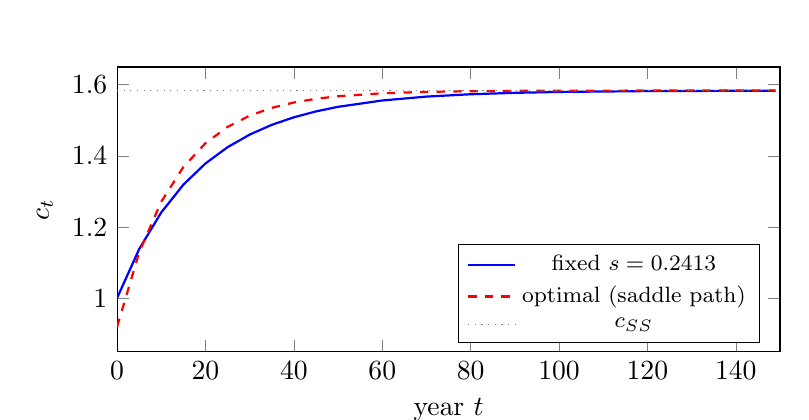
\begin{tikzpicture}\begin{axis}[width=10cm,height=5.2cm,xlabel={year $t$},ylabel={$c_t$},legend pos=south east,
legend style={font=\footnotesize},xmin=0,xmax=150,ymin=0.85,ymax=1.65]
\addplot[blue,thick] coordinates {(0,1.0012) (5,1.1389) (10,1.2417) (15,1.3196) (20,1.3791) (25,1.4248) (30,1.4601) (35,1.4875) (40,1.5087) (45,1.5252) (50,1.5381) (60,1.5559) (70,1.5668) (80,1.5734) (90,1.5774) (100,1.5799) (120,1.5823) (149,1.5834)};
\addplot[red,thick,dashed] coordinates {(0,0.9206) (5,1.1297) (10,1.2719) (15,1.3691) (20,1.4359) (25,1.4818) (30,1.5134) (35,1.5352) (40,1.5502) (45,1.5606) (50,1.5678) (60,1.5761) (70,1.5801) (80,1.5820) (90,1.5830) (100,1.5834) (120,1.5837) (149,1.5838)};
\addplot[gray,dotted] coordinates {(0,1.5838) (150,1.5838)};
\legend{fixed $s=0.2413$, optimal (saddle path), $c_{SS}$}
\end{axis}\end{tikzpicture}\end{center}
The optimal economy consumes less at first and more later; the paths cross between years 5 and 6.
\passo{9.12(d)}{With $\sigma=2$, $u(c)=\frac{c^{-1}}{-1}=-1/c$. Discounted utility of a path:}
\begin{equation}
U=\sum_{t=0}^{149}0.95^t u(c_t). \label{q6:U}
\end{equation}
Evaluating \eqref{q6:U} on the two paths of (c):
\[
U^{\text{fixed}}=-15.79988,\qquad U^{\text{opt}}=-15.74360 ;
\]
the optimal path is better.
\passo{9.12(e)}{Scaling every $c_t$ by $\lambda$ multiplies each $u(c_t)$ in \eqref{q6:U}, and so $U$, by $\lambda^{1-\sigma}$:}
\begin{equation}
U(\lambda c)=\lambda^{1-\sigma}U(c)=\lambda^{-1}U(c). \label{q6:scale}
\end{equation}
Using \eqref{q6:scale}, solve $\lambda^{-1}U^{\text{opt}}=U^{\text{fixed}}$:
\[
\lambda=\frac{U^{\text{opt}}}{U^{\text{fixed}}}=\frac{(-15.74360)}{(-15.79988)}=0.996438,
\]
a cut of $1-\lambda=0.356\%$ of consumption.
\passo{(f) golden rule}{$s=0.2413<s_{GR}=\alpha=0.40$. Rewrite \eqref{q6:IY}:}
\[
\frac IY=\alpha\cdot\frac{\delta}{\rho+\delta},\qquad \frac{\delta}{\rho+\delta}<1\iff\rho>0 .
\]
$K_{GR}$ maximises steady-state consumption $K^\alpha-\delta K$, so it solves
\begin{equation}
F_K=\alpha K_{GR}^{\alpha-1}=\delta. \label{q6:gr}
\end{equation}
Solve \eqref{q6:gr} as in 9.11(a):
\[
K_{GR}=(\alpha/\delta)^{\frac1{1-\alpha}}=\big((0.4)/(0.08)\big)^{\frac1{1-(0.4)}}=5^{1/0.6}=14.62>K_{SS}=6.30 .
\]
Comparing \eqref{q6:gr} with \eqref{q6:mgr}, the gap closes only as $\beta\to1$ ($\rho\to0$).
\intuicao{The right constant saving rate costs only a third of a percent of consumption: Solow's assumption is cheap when $s$ is the
equilibrium's long-run rate. That rate is set by impatience, not by the golden rule.}
\refbib{Kurlat (2020), \S9.3, eqs.\ (9.3.13)--(9.3.17), pp.~172--178; \S4.3, eq.\ (4.3.4). Numbers match the project's solution
\texttt{Resolucao/}\allowbreak\texttt{kurlat\_solutions\_ch09.tex}, Problems 9.11--9.12 ($c_0=0.9206271904$, $\lambda=0.996438$). The instructor's PSET~5 covers
the Euler equation and arbitrage of the same economy (Lista 5, Q2) but stops before the steady state.}
\rubrica{
\item 9.11 closed forms: 3 pts. 9.12(a)--(b) with a correct shooting rule: 4 pts; $c_0$ guessed rather than found: max.\ 1 pt for (b).
\item (c)--(e): 3 pts. (f): 2 pts. Ceiling: claiming $K_{SS}=K_{GR}$ ``because of the First Welfare Theorem'': 0 for (f).
}
\end{sol}

% -----------------------------------------------------------------------------
\questao{(9 points) \textit{Source: Romer, D. (2012), \emph{Advanced Macroeconomics}, 4th ed., Problem 2.16 ``Depreciation in the
Diamond model and microeconomic foundations for the Solow model'', p.~97 --- statement reproduced verbatim, all items (a)--(b), preceded
by the set-up and part (a) of Problem 2.15, p.~97, which 2.16(b) refers to (2.15(b)--(d) omitted); item (c) is added by this list.}
\emph{Harder, contrast.} \emph{What this trains:} the exam's ``Solow with $\delta=1$'' remark done right, in
the overlapping-generations reading where the young save only their wage.}

\noindent\textit{Added (not in the book): Problem 2.15 is included because 2.16(b) refers to it.}\par

\noindent\textbf{2.15.} \emph{A discrete-time version of the Solow model.} Suppose $Y_t=F(K_t,A_tL_t)$, with
$F(\bullet)$ having constant returns to scale and the intensive form of the production function satisfying the Inada conditions.
Suppose also that $A_{t+1}=(1+g)A_t$, $L_{t+1}=(1+n)L_t$, and $K_{t+1}=K_t+sY_t-\delta K_t$.
\begin{enumerate}[label=(\alph*),leftmargin=2.2em,topsep=2pt,itemsep=1pt]
\item Find an expression for $k_{t+1}$ as a function of $k_t$.
\end{enumerate}

\noindent\textbf{2.16.} \emph{Depreciation in the Diamond model and microeconomic foundations for the Solow model.} Suppose that in the Diamond model capital depreciates at rate $\delta$, so that $r_t=f'(k_t)-\delta$.
\begin{enumerate}[label=(\alph*),leftmargin=2.2em,topsep=2pt,itemsep=1pt]
\item How, if at all, does this change in the model affect equation (2.59) giving $k_{t+1}$ as a function of $k_t$?
\item In the special case of logarithmic utility, Cobb--Douglas production, and $\delta=1$, what is the equation for $k_{t+1}$ as a
function of $k_t$? Compare this with the analogous expression for the discrete-time version of the Solow model with $\delta=1$ from
part (a) of Problem 2.15.
\end{enumerate}

\noindent\textit{Added parts (not in the book):}\par\nopagebreak
\textbf{(c)} Compare the implied saving rate with $s_{GR}$ and state when this economy over-accumulates.
\resolespaco
\begin{sol}
\begin{notacao}
\item $C_{1t}$, $C_{2t+1}$: consumption of generation $t$ when young and when old. $\rho>-1$: discount rate, $\beta\equiv\frac1{1+\rho}$.
\item $A_t$, $L_t$: technology and number of young, growing at rates $g$ and $n$. $k\equiv K/(AL)$: capital per effective worker;
$f(k)$: intensive production function, $f'>0$, $f''<0$; Cobb--Douglas $f(k)=k^\alpha$, $\alpha\in(0,1)$.
\item $w_t$: wage per effective worker. $r_{t+1}$: interest rate. $\delta\in[0,1]$: depreciation.
\item $s(r)$: share of the wage the young save. $s_S$: Solow's saving rate that reproduces the same law of motion. $s_{GR}$: golden-rule rate.
\end{notacao}
\passo{(a)}{Young at $t$ maximise $\ln C_{1t}+\beta\ln C_{2t+1}$ subject to}
\begin{equation}
C_{1t}+\frac{C_{2t+1}}{1+r_{t+1}}=A_tw_t. \label{q7:pv}
\end{equation}
\eqref{q7:pv} does not contain $\delta$, so the saving rule $s(r_{t+1})$ out of the wage is unchanged by depreciation. Only the return
changes:
\begin{equation}
r_{t+1}=f'(k_{t+1})-\delta. \label{q7:r}
\end{equation}
Market clearing: next period's capital is the young's saving,
\begin{equation}
K_{t+1}=s(r_{t+1})A_tw_tL_t. \label{q7:mc}
\end{equation}
The competitive wage per effective worker is
\begin{equation}
w=f(k)-kf'(k). \label{q7:w}
\end{equation}
Divide \eqref{q7:mc} by $A_{t+1}L_{t+1}=(1+n)(1+g)A_tL_t$, then substitute \eqref{q7:r} and \eqref{q7:w}:
\begin{align}
k_{t+1} &= \frac{s(r_{t+1})A_tw_tL_t}{\big((1+n)(1+g)A_tL_t\big)}\nonumber\\
&= \frac{s(r_{t+1})\,w_t}{(1+n)(1+g)}\nonumber\\
&= \frac{s(f'(k_{t+1})-\delta)\,[f(k_t)-k_tf'(k_t)]}{(1+n)(1+g)}. \label{q7:lom}
\end{align}
In \eqref{q7:lom} depreciation matters only through $s(\cdot)$: in the log case not at all.
\passo{(b)}{Log utility: the young save the share $\frac{\beta}{1+\beta}$ of the wage. Substitute $\beta=\frac1{1+\rho}$:}
\begin{align}
s &= \frac{\big(1/(1+\rho)\big)}{1+\big(1/(1+\rho)\big)}\nonumber\\
&= \frac{1/(1+\rho)}{(2+\rho)/(1+\rho)}\nonumber\\
&= \frac1{2+\rho}, \label{q7:s}
\end{align}
independent of $r$. Cobb--Douglas in \eqref{q7:w}:
\begin{align}
w &= \big(k^\alpha\big)-k\big(\alpha k^{\alpha-1}\big)\nonumber\\
&= k^\alpha-\alpha k^\alpha=(1-\alpha)k^\alpha. \label{q7:wcd}
\end{align}
Substitute \eqref{q7:s} and \eqref{q7:wcd} into \eqref{q7:lom}:
\begin{align}
k_{t+1} &= \frac{\big(\frac1{2+\rho}\big)\big((1-\alpha)k_t^\alpha\big)}{(1+n)(1+g)}\nonumber\\
&= \frac{(1-\alpha)k_t^\alpha}{(2+\rho)(1+n)(1+g)}. \label{q7:lomlog}
\end{align}
Solow 2.15(a) with $\delta=1$:
\begin{equation}
k_{t+1}=\frac{s_Sk_t^\alpha}{(1+n)(1+g)}. \label{q7:solow}
\end{equation}
\eqref{q7:lomlog} and \eqref{q7:solow} are identical with
\begin{align}
s_S &= \frac{1-\alpha}{2+\rho}\nonumber\\
&= \frac{1-\alpha}{2+\big(\frac1\beta-1\big)}\nonumber\\
&= \frac{(1-\alpha)\beta}{1+\beta}: \label{q7:sS}
\end{align}
the young's saving of their wage is the whole gross saving, since with $\delta=1$ the old hold no capital to run down.
\passo{(c)}{Golden rule: $s_{GR}=\alpha$ (Question~2, \eqref{q2:sgr}). Over-accumulation means \eqref{q7:sS} exceeds it. Multiply by
$1+\beta$ and collect terms:}
\begin{align*}
\frac{(1-\alpha)\beta}{1+\beta} &> \alpha\\
\beta-\alpha\beta &> \alpha+\alpha\beta\\
\beta(1-2\alpha) &> \alpha.
\end{align*}
As $\beta<1$, the left side is below $1-2\alpha$, so this needs $1-2\alpha>\alpha$, i.e.\ $\alpha<\frac13$. E.g.\ $\alpha=0.2$, $\beta=0.9$:
\[
s_S=\frac{(1-0.2)(0.9)}{1+(0.9)}=0.8\times0.9/1.9=0.379>0.2 .
\]
Unlike Kurlat's infinite-horizon economy (Q6(f)), finite lives can put the equilibrium above the golden rule.
\intuicao{Diamond microfounds Solow's constant $s$ only in a knife-edge case (log, Cobb--Douglas, $\delta=1$), and the saving rate it
delivers comes from preferences and the wage share, not from any golden-rule calculation.}
\refbib{Romer (2012), \S\S2.9--2.11, eq.\ (2.60), pp.~78--91; Romer, \emph{Solution Manual}, Problems 2.15 and 2.16: same law of motion,
$s(r)=1/(2+\rho)$ and aggregate saving rate $(1-\alpha)/(2+\rho)$. Kurlat (2020), \S9.1 (two-period equilibrium).}
\rubrica{
\item (a) market clearing $K_{t+1}=$ young's saving and the role of $\delta$ through $r$ only: 3 pts.
\item (b) law of motion and the identification $s_S=(1-\alpha)\beta/(1+\beta)$: 4 pts; $s_S=\beta/(1+\beta)$ (forgetting that only wages are saved): max.\ 2 pts.
\item (c): 2 pts.
}
\end{sol}

% -----------------------------------------------------------------------------
\questao{(10 points) \emph{Conceptual, words only.} True or false? Justify each in at most four lines, without algebra.}

\textbf{a)} (2 points) In the exam's economy (log utility over $c_1,c_2$; one unit of time; work carries no disutility; $w_1>0$), no
first-order condition for $L_1$ exists, so $L_1$ is left undetermined.
\gabarito{F}
\begin{sol}
\begin{notacao}
\item $L_1\in[0,1]$: hours worked in period 1. $w_1>0$: wage. $\mathcal L$: the household's Lagrangian.
\item $\lambda>0$: multiplier on the budget (utility value of one unit of resources). $\nu\ge0$: multiplier on $L_1\le1$.
\end{notacao}
\passo{why}{$L_1$ is not in utility but it is in the budget: an extra hour adds $w_1$ to resources, worth $\lambda w_1>0$ in utility. The
marginal gain is positive at every $L_1<1$, so the constraint $L_1\le1$ binds: $L_1=1$, a corner. Stating ``$\partial\mathcal L/\partial L_1=\lambda w_1-\nu=0$
with $\nu>0$, hence $L_1=1$'' \emph{is} the FOC. With leisure in utility it becomes interior (Q9).}
\end{sol}

\textbf{b)} (2 points) With $u=\ln c$ the saving rate does not depend on $r$; so in Kurlat 6.2 a rate cut leaves every person's
$s=(y-c)/y$ unchanged.
\gabarito{F}
\begin{sol}
\begin{notacao}
\item $y_1,y_2\ge0$: income in periods 1 and 2; $c_1$: period-1 consumption; $s=(y-c)/y$: saving out of current income.
\item $r>-1$: interest rate. $\beta\in(0,1)$: discount factor.
\end{notacao}
\passo{why}{Log makes saving a constant share $\frac\beta{1+\beta}$ of \emph{lifetime wealth}, and $c_1$ independent of $r$ only when all resources
arrive in period 1 (the exam). With future income, wealth $y_1+\frac{y_2}{1+r}$ rises when $r$ falls, so $c_1$ rises and $s$ out of current
income falls: strongly for residents, hardly for athletes.}
\end{sol}

\textbf{c)} (2 points) The First Welfare Theorem holds in Kurlat's infinite-horizon economy, so its steady state is the golden rule.
\gabarito{F}
\begin{sol}
\begin{notacao}
\item $F_K$: marginal product of capital. $\delta\in(0,1)$: depreciation. $\rho>0$: rate of time preference.
\item $K_{SS}$: steady-state capital ($F_K=\rho+\delta$); $K_{GR}$: golden-rule capital ($F_K=\delta$).
\end{notacao}
\passo{why}{The golden rule maximises consumption \emph{in the steady state}, ignoring the cost of getting there. Reaching it means giving up
consumption now for gains later, which impatient households value less. Efficiency is relative to their preferences: the modified
golden rule $F_K=\rho+\delta>\delta$ puts $K_{SS}$ below $K_{GR}$. No contradiction.}
\end{sol}

\textbf{d)} (2 points) An economy with capital above the golden rule is dynamically inefficient: a permanently lower saving rate raises
consumption at every date, starting today.
\gabarito{T}
\begin{sol}
\begin{notacao}
\item $s$: saving rate. $k$: capital per (effective) worker; $k_{GR}$: its golden-rule level.
\item $r$: interest rate. $n$, $g$: growth rates of population and technology.
\end{notacao}
\passo{why}{Cutting $s$ raises consumption at once; as capital falls toward $k_{GR}$, steady-state consumption rises (it falls in $k$ above
$k_{GR}$), so no date loses. Equivalently $r<n$ ($+g$). This Pareto improvement cannot exist in Kurlat's economy (Q6(f)) but can in
overlapping generations (Q7(c), Q10), where infinitely many generations break the welfare theorem.}
\end{sol}

\textbf{e)} (2 points) Once the household's rule $a_1=\frac{\beta}{1+\beta}\times$(resources) is known, the economy's law of motion $k_2=\phi(k_1)$
follows without further conditions.
\gabarito{F}
\begin{sol}
\begin{notacao}
\item $a_1$: the household's saving (assets carried to period 2). $k_1$, $k_2$ ($K_1$, $K_2$): capital in periods 1 and 2;
$\phi$: the law of motion $k_2=\phi(k_1)$.
\item $w_1$: wage. $\Pi_1$: profit paid to the household that owns the firm. $Y_1$: period-1 output.
\end{notacao}
\passo{why}{$a_1$ is a demand for assets at given prices. Three more pieces are needed: firm FOCs that turn $k_1$ into $w_1$ and $\Pi_1$
(resources $=Y_1$ when the household owns the firm), market clearing $K_2=a_1$ (capital is the only asset), and the period timing. Only
then is saving a law of motion.}
\end{sol}
\begin{sol}
\rubrica{
\item Each item: 0.5 for the verdict, 1.5 for the reason. A right verdict with a wrong reason: 0.5.
}
\end{sol}

% =============================================================================
\bloco{3}{Created: the exam's economy, extended}{Kurlat \S\S6.2, 7.1, 9.1, 4.3; Romer \S2.9--2.11 \,\textbullet\, 28 points}

\questao{(15 points) \emph{The exam's household with leisure, inside an economy.} Periods $t=1,2,\dots$ Each period a generation of
size one is born and lives two periods, with one unit of time when young and none when old. Generation $t$ maximises
$\ln c_{1t}+\psi\ln(1-L_t)+\beta\ln c_{2t+1}$, $\psi>0$, $0<\beta<1$. Technology $Y_t=AK_t^\alpha L_t^{1-\alpha}$, $\delta=1$, competitive markets; saving is lent
to firms as next period's capital and earns $1+r_{t+1}=r^K_{t+1}$. \emph{Generation 1 is the exam's household:} it is born with assets
$a_0\ge0$ and owns the firm, which owns $K_1>0$, so in period 1 it receives the profit $\Pi_1=Y_1-w_1L_1$ besides its wage. From
period 2 on, the old rent their capital to firms, which earn zero profit; each young generation earns only its wage.}

\textbf{a)} (2 points) Write generation 1's two period budgets and its present-value budget constraint. List every choice variable
and every income source, and read the constraint in words.

\textbf{b)} (4 points) Derive all first-order conditions and closed forms for $c_1,c_2,L_1,a_1$ given $(w_1,\Pi_1,r_2,a_0)$. When is $L_1$
interior? Show that $a_1$ is the share $\frac{\beta}{1+\beta}$ of the resources $a_0+w_1L_1+\Pi_1$. What happens as $\psi\to0$?

\textbf{c)} (3 points) Let $a_0=0$. Using the firm's FOC, find equilibrium $L_1^\ast$ (show it depends on neither $K_1$ nor $A$) and the
map $K_2=\phi_1(K_1)$.

\textbf{d)} (3 points) For $t\ge2$ find the young's labour $\bar L$, the law of motion $K_{t+1}=\phi(K_t)$, the steady state and its stability.
Draw $\phi$ against the $45^\circ$ line for $\alpha=1/3$, $\beta=0.8$, $\psi=0.5$, $A=5$, $K_1=1$, marking $K^\ast$ and the path from $K_2$.

\textbf{e)} (3 points) Compare with Solow ($\delta$, $n$, $s$) and with $s_{GR}$. When does this economy over-accumulate? Evaluate for
$(\alpha,\beta)=(1/3,0.8)$ and $(0.2,0.9)$, with the interest rate in each. Why does generation 1 work less than later ones, and what goes
wrong if $\Pi_1$ is left out of its budget?
\resolespaco
\begin{sol}
\begin{notacao}
\item $c_{1t}$, $c_{2t+1}>0$: consumption of generation $t$ young and old (for generation 1: $c_1$, $c_2$). $L_t\in[0,1]$: hours of the
young; $1-L_t$: leisure. $\psi>0$: weight of leisure. $\beta\in(0,1)$: discount factor.
\item $Y_t=AK_t^\alpha L_t^{1-\alpha}$: output, $A>0$, $\alpha\in(0,1)$; $K_t$: capital, $\delta=1$.
\item $w_t$: wage. $r_{t+1}$: interest rate, $1+r_{t+1}=r^K_{t+1}$ (rental rate). $a_0\ge0$: generation 1's initial assets.
$a_1$ ($a_t$): saving of generation 1 ($t$). $\Pi_1=Y_1-w_1L_1$: period-1 profit.
\item $X$: full wealth; $R$: resources; $\lambda>0$: multiplier on the budget (defined where first used).
\item $L_1^\ast$: generation 1's equilibrium hours; $\bar L$: later generations' hours. $\phi_1$, $\phi$: laws of motion of capital;
$K^\ast$: steady state. $s_{eq}$: the equilibrium saving rate $K_{t+1}/Y_t$. $s_{GR}$: golden-rule rate.
\end{notacao}
\passo{(a)}{The two period budgets of generation 1:}
\begin{align}
c_1+a_1 &= a_0+w_1L_1+\Pi_1, \label{q9:b1}\\
c_2 &= (1+r_2)a_1. \label{q9:b2}
\end{align}
Solve \eqref{q9:b2} for $a_1=\frac{c_2}{1+r_2}$ and substitute into \eqref{q9:b1}:
\begin{equation}
c_1+\frac{c_2}{1+r_2}=a_0+w_1L_1+\Pi_1. \label{q9:pv}
\end{equation}
Add $w_1(1-L_1)$ to both sides of \eqref{q9:pv}:
\begin{equation}
c_1+\frac{c_2}{1+r_2}+w_1(1-L_1)=a_0+w_1+\Pi_1\equiv X. \label{q9:full}
\end{equation}
Choices: $c_1,c_2,a_1,L_1$ with $0\le L_1\le1$. Income: initial wealth, labour, \emph{and profits}. Reading: the present value of
consumption plus the value of leisure equals full wealth (time valued at $w_1$).
\passo{(b) FOCs}{The Lagrangian, with the budget \eqref{q9:pv}:}
\begin{equation}
\mathcal L=\ln c_1+\psi\ln(1-L_1)+\beta\ln c_2+\lambda\Big[a_0+w_1L_1+\Pi_1-c_1-\frac{c_2}{1+r_2}\Big]. \label{q9:lag}
\end{equation}
Differentiate \eqref{q9:lag} with respect to $c_1$, $c_2$ and $L_1$:
\begin{align}
\frac1{c_1} &= \lambda, \label{q9:f1}\\
\frac\beta{c_2} &= \frac\lambda{1+r_2}, \label{q9:f2}\\
\frac\psi{1-L_1} &= \lambda w_1. \label{q9:f3}
\end{align}
Substitute \eqref{q9:f1} into \eqref{q9:f2} (Euler) and into \eqref{q9:f3} (labour supply):
\begin{align}
\frac\beta{c_2} &= \frac{(1/c_1)}{1+r_2}\nonumber\\
c_2 &= \beta(1+r_2)c_1, \label{q9:euler}\\
\frac\psi{1-L_1} &= \Big(\frac1{c_1}\Big)w_1\nonumber\\
w_1(1-L_1) &= \psi c_1. \label{q9:ls}
\end{align}
\passo{(b) closed forms}{Substitute \eqref{q9:euler} and \eqref{q9:ls} into the full budget \eqref{q9:full}:}
\begin{align*}
c_1+\frac{\big(\beta(1+r_2)c_1\big)}{1+r_2}+(\psi c_1) &= X\\
c_1+\beta c_1+\psi c_1 &= X,
\end{align*}
so
\begin{equation}
c_1=\frac{X}{1+\beta+\psi}. \label{q9:c1}
\end{equation}
Substitute \eqref{q9:c1} into \eqref{q9:euler}, into \eqref{q9:ls} solved for $L_1$, and into $a_1=\frac{c_2}{1+r_2}$:
\begin{align}
c_2 &= \beta(1+r_2)\Big(\frac{X}{1+\beta+\psi}\Big)\nonumber\\
&= \frac{\beta(1+r_2)X}{1+\beta+\psi}, \nonumber\\
L_1 &= 1-\frac{\psi}{w_1}\Big(\frac{X}{1+\beta+\psi}\Big)\nonumber\\
&= 1-\frac{\psi X}{(1+\beta+\psi)w_1}, \label{q9:L1}\\
a_1 &= \frac1{1+r_2}\Big(\frac{\beta(1+r_2)X}{1+\beta+\psi}\Big)\nonumber\\
&= \frac{\beta X}{1+\beta+\psi}. \label{q9:a1}
\end{align}
Interior iff $L_1>0$. By \eqref{q9:L1} and the definition of $X$ in \eqref{q9:full}:
\begin{align}
L_1>0 &\iff 1-\frac{\psi(a_0+w_1+\Pi_1)}{(1+\beta+\psi)w_1}>0\nonumber\\
&\iff \psi(a_0+w_1+\Pi_1)<(1+\beta+\psi)w_1\nonumber\\
&\iff \psi(a_0+\Pi_1)<(1+\beta)w_1. \label{q9:int}
\end{align}
\passo{(b) saving share}{Resources are full wealth minus the value of leisure, \eqref{q9:full}; then use \eqref{q9:ls} and \eqref{q9:c1}:}
\begin{align}
R\equiv a_0+w_1L_1+\Pi_1 &= X-w_1(1-L_1)\nonumber\\
&= X-(\psi c_1)\nonumber\\
&= X-\psi\Big(\frac{X}{1+\beta+\psi}\Big)\nonumber\\
&= X-\frac{\psi X}{1+\beta+\psi}\nonumber\\
&= \frac{(1+\beta)X}{1+\beta+\psi}. \label{q9:R}
\end{align}
Divide \eqref{q9:a1} by \eqref{q9:R}:
\begin{align*}
\frac{a_1}{R} &= \frac{\big(\beta X/(1+\beta+\psi)\big)}{\big((1+\beta)X/(1+\beta+\psi)\big)}\\
&= \frac{\beta}{1+\beta},
\end{align*}
the exam's rate, for any $\psi$ and any $r_2$. As $\psi\to0$, \eqref{q9:L1} and \eqref{q9:c1} give
\begin{align*}
L_1 &\to 1-\frac{(0)X}{(1+\beta+(0))w_1}=1\quad\text{(the exam's corner)},\\
c_1 &\to \frac{(a_0+w_1+\Pi_1)}{1+\beta+(0)}=\frac{a_0+w_1+\Pi_1}{1+\beta}.
\end{align*}
\passo{(c) labour}{The firm's FOC for labour, and profit as output minus wages:}
\begin{align}
w_1 &= (1-\alpha)AK_1^\alpha L_1^{-\alpha}=\frac{(1-\alpha)Y_1}{L_1}, \label{q9:w}\\
\Pi_1 &= Y_1-w_1L_1=\alpha Y_1. \label{q9:Pi}
\end{align}
With $a_0=0$, \eqref{q9:full} and \eqref{q9:Pi} give $X=(0)+w_1+(\alpha Y_1)=w_1+\alpha Y_1$. Multiply \eqref{q9:L1} out as
$w_1(1-L_1)=\frac{\psi X}{1+\beta+\psi}$ and substitute \eqref{q9:w} and $X$:
\begin{align*}
\Big(\frac{(1-\alpha)Y_1}{L_1}\Big)(1-L_1) &= \frac{\psi}{1+\beta+\psi}\Big[\Big(\frac{(1-\alpha)Y_1}{L_1}\Big)+\alpha Y_1\Big]\\
\frac{(1-\alpha)Y_1(1-L_1)}{L_1} &= \frac{\psi}{1+\beta+\psi}\Big[\frac{(1-\alpha)Y_1}{L_1}+\alpha Y_1\Big].
\end{align*}
Multiply by $\frac{L_1(1+\beta+\psi)}{Y_1}$:
\[
(1-\alpha)(1+\beta+\psi)(1-L_1)=\psi(1-\alpha)+\psi\alpha L_1 .
\]
Collect the $L_1$ terms on the right; $\psi(1-\alpha)$ cancels on the left:
\[
(1-\alpha)(1+\beta)=L_1\big[(1-\alpha)(1+\beta)+\psi\big].
\]
Hence
\begin{equation}
L_1^\ast=\frac{(1-\alpha)(1+\beta)}{(1-\alpha)(1+\beta)+\psi}. \label{q9:Lstar}
\end{equation}
$Y_1$ cancelled, so $K_1$ and $A$ drop out. Interiority: \eqref{q9:int} with $a_0=0$, then \eqref{q9:w}--\eqref{q9:Pi}, then
\eqref{q9:Lstar}:
\begin{align*}
\psi\Pi_1<(1+\beta)w_1 &\iff \psi(\alpha Y_1)<(1+\beta)\Big(\frac{(1-\alpha)Y_1}{L_1^\ast}\Big)\\
&\iff \psi\alpha L_1^\ast<(1-\alpha)(1+\beta)\\
&\iff \psi\alpha\Big(\frac{(1-\alpha)(1+\beta)}{(1-\alpha)(1+\beta)+\psi}\Big)<(1-\alpha)(1+\beta)\\
&\iff \psi\alpha<(1-\alpha)(1+\beta)+\psi,
\end{align*}
always true.
\passo{(c) map}{With $a_0=0$, \eqref{q9:w}--\eqref{q9:Pi} give $R=w_1L_1+\Pi_1=\big(\frac{(1-\alpha)Y_1}{L_1}\big)L_1+(\alpha Y_1)=Y_1$. Capital is
the only asset, so market clearing is}
\begin{equation}
K_2=a_1. \label{q9:mc}
\end{equation}
Substitute $a_1=\frac{\beta}{1+\beta}R=\frac{\beta}{1+\beta}Y_1$ and $L_1=L_1^\ast$ into \eqref{q9:mc}:
\begin{align}
K_2 &= \Big(\frac{\beta}{1+\beta}Y_1\Big)\nonumber\\
&= \frac{\beta}{1+\beta}\big(AK_1^\alpha(L_1^\ast)^{1-\alpha}\big)\nonumber\\
&= \frac{\beta}{1+\beta}AK_1^\alpha(L_1^\ast)^{1-\alpha}\equiv\phi_1(K_1). \label{q9:phi1}
\end{align}
\passo{(d) later generations}{$a_0=\Pi=0$, so \eqref{q9:full} gives $X=(0)+w_t+(0)=w_t$, and \eqref{q9:L1} becomes}
\begin{align}
\bar L &= 1-\frac{\psi(w_t)}{(1+\beta+\psi)w_t}\nonumber\\
&= 1-\frac{\psi}{1+\beta+\psi}=\frac{1+\beta}{1+\beta+\psi}. \label{q9:Lbar}
\end{align}
Saving is the share $\frac{\beta}{1+\beta}$ of resources $w_t\bar L$, and $w_t\bar L=(1-\alpha)Y_t$ by \eqref{q9:w}:
\begin{equation}
a_t=\frac{\beta}{1+\beta}w_t\bar L=\frac{\beta}{1+\beta}\big((1-\alpha)Y_t\big). \label{q9:at}
\end{equation}
Market clearing $K_{t+1}=a_t$, with $Y_t=AK_t^\alpha\bar L^{1-\alpha}$ in \eqref{q9:at}:
\begin{align}
K_{t+1} &= \frac{\beta}{1+\beta}(1-\alpha)\big(AK_t^\alpha\bar L^{1-\alpha}\big)\nonumber\\
\phi(K) &= \frac{\beta(1-\alpha)}{1+\beta}A\bar L^{1-\alpha}K^\alpha. \label{q9:phi}
\end{align}
$\phi(0)=0$, $\phi'>0$, $\phi''<0$, $\phi'(0^+)=\infty$, $\phi'(\infty)=0$: one positive fixed point. Set $\phi(K)=K$ in \eqref{q9:phi}, divide
by $K^\alpha$ and raise to the power $\frac1{1-\alpha}$:
\begin{align}
\frac{\beta(1-\alpha)}{1+\beta}A\bar L^{1-\alpha}K^\alpha &= (K)\nonumber\\
K^{1-\alpha} &= \frac{\beta(1-\alpha)A\bar L^{1-\alpha}}{1+\beta}\nonumber\\
K^\ast &= \Big[\frac{\beta(1-\alpha)A\bar L^{1-\alpha}}{1+\beta}\Big]^{\frac1{1-\alpha}}. \label{q9:Kstar}
\end{align}
Differentiating \eqref{q9:phi}, $\phi'(K^\ast)=\alpha\frac{\phi(K^\ast)}{K^\ast}=\alpha\frac{(K^\ast)}{K^\ast}=\alpha<1$: monotone, stable.
\passo{(d) numbers}{With $\alpha=1/3$, $\beta=0.8$, $\psi=0.5$, $A=5$, $K_1=1$:}
\begin{align*}
\bar L &= \tfrac{1+0.8}{1+0.8+0.5}=1.8/2.3=0.7826 &&\text{by \eqref{q9:Lbar}},\\
L_1^\ast &= \tfrac{(2/3)(1.8)}{(2/3)(1.8)+0.5}=1.2/1.7=0.7059 &&\text{by \eqref{q9:Lstar}},\\
\phi(K) &= \tfrac{0.8\cdot2/3}{1.8}\cdot5\cdot0.7826^{2/3}K^{1/3}=1.2581K^{1/3} &&\text{by \eqref{q9:phi}},\\
K^\ast &= 1.2581^{1.5}=1.4112 &&\text{by \eqref{q9:Kstar}},\\
Y_1 &= 5\cdot(1)^{1/3}\cdot0.7059^{2/3}=3.9639,\\
K_2 &= \tfrac{0.8}{1.8}\times3.9639=1.7617 &&\text{by \eqref{q9:phi1}}.
\end{align*}
Then \eqref{q9:phi} gives $K_3=1.2581\,(1.7617)^{1/3}=1.5195$ and, iterating the same way, $K_4=1.4464$, $K_5=1.4228\to K^\ast$.
\begin{center}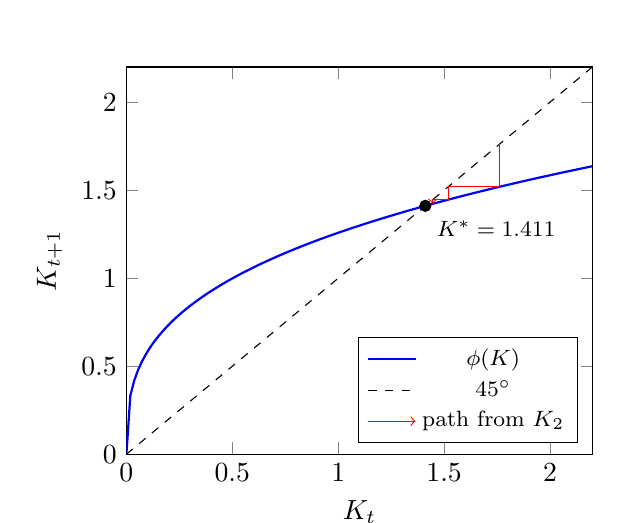
\begin{tikzpicture}\begin{axis}[width=7.5cm,height=6.5cm,xmin=0,xmax=2.2,ymin=0,ymax=2.2,xlabel={$K_t$},ylabel={$K_{t+1}$},
legend pos=south east,legend style={font=\footnotesize},samples=120,domain=0:2.2]
\addplot[blue,thick] {1.2581*x^(1/3)};
\addplot[black,dashed] {x};
\addplot[red,thin,->] coordinates {(1.7617,1.7617) (1.7617,1.5195) (1.5195,1.5195) (1.5195,1.4464) (1.4464,1.4464) (1.4464,1.4228)};
\addplot[only marks,mark=*] coordinates {(1.4112,1.4112)};
\legend{$\phi(K)$, $45^\circ$, path from $K_2$}
\node[anchor=north west,font=\footnotesize] at (axis cs:1.42,1.38) {$K^\ast=1.411$};
\end{axis}\end{tikzpicture}\end{center}
\passo{(e) Solow}{With $\delta=1$, $n=0$ Solow's law of motion is}
\begin{equation}
K_{t+1}=sY_t. \label{q9:solow}
\end{equation}
Here, by market clearing and \eqref{q9:at},
\begin{equation}
\frac{K_{t+1}}{Y_t}=\frac{\beta(1-\alpha)}{1+\beta}\equiv s_{eq}: \label{q9:seq}
\end{equation}
the same law of motion as \eqref{q9:solow}, but $s$ is chosen (patience, and the wage share because only wages are saved), and it
need not be $s_{GR}=\alpha$. Golden rule: MPK $=n+\delta=1$. At $K^\ast$, $K=s_{eq}Y$ by \eqref{q9:seq}, so
\begin{align}
1+r=\text{MPK} &= \alpha\frac YK\nonumber\\
&= \alpha\frac{Y}{(s_{eq}Y)}\nonumber\\
&= \frac{\alpha}{s_{eq}}. \label{q9:r}
\end{align}
By \eqref{q9:r}, and multiplying out \eqref{q9:seq} as in Question~7(c):
\begin{align*}
r<0=n &\iff s_{eq}>\alpha\\
&\iff \frac{\beta(1-\alpha)}{1+\beta}>\alpha\\
&\iff \beta(1-2\alpha)>\alpha .
\end{align*}
\passo{(e) numbers}{Using \eqref{q9:seq} and \eqref{q9:r}:}
\begin{align*}
(1/3,0.8) &: \ s_{eq}=\tfrac{0.8\times2/3}{1.8}=0.2963<0.3333,\quad 1+r=\tfrac{1/3}{0.2963}=1.125,\quad r=0.125>0,\\
(0.2,0.9) &: \ s_{eq}=\tfrac{0.9\times0.8}{1.9}=0.3789>0.2,\quad 1+r=\tfrac{0.2}{0.3789}=0.5278,\quad r=-0.472<0.
\end{align*}
The first is under-accumulation, efficient; the second is over-accumulation, dynamically inefficient.
\passo{(e) profits}{Compare \eqref{q9:Lstar} with \eqref{q9:Lbar}; cross-multiply and cancel $(1-\alpha)(1+\beta)$:}
\begin{align*}
L_1^\ast<\bar L &\iff \frac{(1-\alpha)(1+\beta)}{(1-\alpha)(1+\beta)+\psi}<\frac{1+\beta}{1+\beta+\psi}\\
&\iff (1-\alpha)(1+\beta+\psi)<(1-\alpha)(1+\beta)+\psi\\
&\iff (1-\alpha)\psi<\psi,
\end{align*}
true. Profits are non-labour income; the wealth effect buys leisure. Dropping $\Pi_1$ gives $L_1=\bar L$ and
$K_2=\frac{\beta}{1+\beta}(1-\alpha)Y_1$: it understates resources by $\alpha Y_1$ and overstates labour.
\intuicao{The household rule is the same in every generation; what differs is who owns what. Market clearing turns that rule into
$\phi$, and the saving rate it implies answers to preferences and factor shares, not to the golden rule.}
\refbib{Kurlat (2020), \S6.2 (Euler), \S7.1 (labour supply), \S9.1 (two-period equilibrium), \S4.3 (golden rule); Romer (2012), \S\S2.9--2.11.
Same structure as Prova 01, Q2(c)--(f), with $\psi=0$; see \texttt{Prova/prova-01-error-analysis.md}.}
\rubrica{
\item (a): 2 pts; $\Pi_1$ missing: max.\ 1 pt. (b) all four FOCs (or three plus the corner argument): 2 pts; closed forms and $\beta/(1+\beta)$: 2 pts.
\item (c): 3 pts. (d): 3 pts, of which the diagram 1 pt (axes, $45^\circ$ line, curve, $K^\ast$ and direction marked separately: 0.25 each).
\item (e): 3 pts. Ceiling: no market clearing ($K_{t+1}=a_t$) anywhere: max.\ 6 pts for the whole question.
}
\end{sol}

% -----------------------------------------------------------------------------
\questao{(13 points) \emph{CRRA and population growth: when the saving rate depends on $r$.} Overlapping generations as in
Question~9 but without leisure: each young person supplies one unit of labour, earns only the wage, and the number of young grows,
$L_{t+1}=(1+n)L_t$. Utility $u(c_{1t})+\beta u(c_{2t+1})$ with $u(c)=\frac{c^{1-\sigma}}{1-\sigma}$; $y=Ak^\alpha$ per young worker; $\delta=1$.}

\textbf{a)} (3 points) Solve the young's problem. Show that saving is a share $s(r)$ of the wage, find $s(r)$, and sign $s'(r)$.
Explain the sign through income and substitution effects.

\textbf{b)} (3 points) Using the firm's FOCs and market clearing $K_{t+1}=L_ta_t$, write the law of motion for $k\equiv K/L$. Show that $k_{t+1}$
is unique given $k_t$ when $\sigma\le1$, and give it in closed form for $\sigma=1$.

\textbf{c)} (3 points) Show that the steady state satisfies $s(r)(1+r)=\frac{\alpha(1+n)}{1-\alpha}$ and that the aggregate saving rate is
$\frac{I}{Y}=\frac{\alpha(1+n)}{1+r}$. Conclude: $\frac IY>s_{GR}\iff r<n\iff k^\ast>k_{GR}$.

\textbf{d)} (2 points) Let $\alpha=0.2$, $\beta=0.5$, $n=0.3$, $A=5$. For $\sigma=1$ find $r^\ast$, $k^\ast$, $k_{GR}$ and steady-state consumption per
worker at both. For $\sigma\in\{1/2,2\}$ find $r^\ast$ numerically (Python) and say which economies are dynamically inefficient, and why
$\sigma$ matters.

\textbf{e)} (2 points) Draw the $\sigma=1$ map against the $45^\circ$ line, marking $k^\ast$ and $k_{GR}$. In what sense is this ``Solow with $\delta=1$''?
\resolespaco
\begin{sol}
\begin{notacao}
\item $c_1$, $c_2>0$: consumption young and old. $w$: wage. $a$: saving of a young person. $r>-1$: interest rate; $r^K$: rental rate.
\item $u(c)=\frac{c^{1-\sigma}}{1-\sigma}$, $\sigma>0$ ($1/\sigma$: intertemporal elasticity). $\beta\in(0,1)$: discount factor.
\item $D$: the consumption divisor, as in Question~3, \eqref{q3:D}. $s(r)$: share of the wage saved.
\item $L_t$: number of young, growing at rate $n>-1$. $k\equiv K/L$: capital per young worker; $y=Ak^\alpha$, $A>0$, $\alpha\in(0,1)$;
$\delta=1$.
\item $I/Y$: aggregate saving (investment) rate. $k^\ast$, $r^\ast$: steady state. $k_{GR}$, $s_{GR}$: golden rule. $H(r)$: the
steady-state residual of (d). $\phi(k)$: the law of motion; $s_S$: Solow's saving rate that reproduces it.
\end{notacao}
\passo{(a)}{The young person's two budgets:}
\begin{align}
c_1+a &= w, \label{q10:b1}\\
c_2 &= (1+r)a. \label{q10:b2}
\end{align}
The Euler equation is \eqref{q3:euler}, $c_2=[\beta(1+r)]^{1/\sigma}c_1$. Eliminating $a$ from \eqref{q10:b1}--\eqref{q10:b2} gives the PV
budget
\begin{equation}
c_1+\frac{c_2}{1+r}=w. \label{q10:pv}
\end{equation}
\eqref{q10:pv} is \eqref{q3:pv} with $W=w$, so, as in \eqref{q3:c1},
\begin{equation}
c_1=\frac wD,\qquad D=1+\beta^{1/\sigma}(1+r)^{\frac1\sigma-1}. \label{q10:c1}
\end{equation}
Substitute \eqref{q10:c1} into \eqref{q10:b1}:
\begin{align}
\Big(\frac wD\Big)+a &= w\nonumber\\
a &= w-\frac wD=s(r)w, \label{q10:a}
\end{align}
with
\begin{align}
s(r) &= \frac{D-1}{D}\nonumber\\
&= \frac{\big(1+\beta^{1/\sigma}(1+r)^{\frac1\sigma-1}\big)-1}{\big(1+\beta^{1/\sigma}(1+r)^{\frac1\sigma-1}\big)}\nonumber\\
&= \frac{\beta^{1/\sigma}(1+r)^{\frac1\sigma-1}}{1+\beta^{1/\sigma}(1+r)^{\frac1\sigma-1}}. \label{q10:s}
\end{align}
Write \eqref{q10:s} as $s=1-1/D$ and differentiate, with $D'(r)$ from \eqref{q3:Dr}:
\begin{equation}
s'(r)=\frac{D'(r)}{D^2},\qquad D'(r)=\beta^{1/\sigma}\Big(\frac1\sigma-1\Big)(1+r)^{\frac1\sigma-2}. \label{q10:ds}
\end{equation}
The sign of \eqref{q10:ds} is the sign of $1-\sigma$. The young are pure savers: a higher $r$ makes them richer ($c_1\uparrow$, saving
$\downarrow$) and makes waiting cheaper (saving $\uparrow$). $\sigma<1$: substitution wins; $\sigma>1$: income wins; $\sigma=1$:
\eqref{q10:s} gives
\begin{align*}
s &= \frac{\beta^{1/(1)}(1+r)^{\frac1{(1)}-1}}{1+\beta^{1/(1)}(1+r)^{\frac1{(1)}-1}}\\
&= \frac\beta{1+\beta},
\end{align*}
independent of $r$.
\passo{(b)}{The firm's FOCs, with $\delta=1$ so that $1+r=r^K$:}
\begin{align}
w_t &= (1-\alpha)Ak_t^\alpha, \label{q10:w}\\
1+r_{t+1} &= r^K_{t+1}=\alpha Ak_{t+1}^{\alpha-1}. \label{q10:r}
\end{align}
Market clearing:
\begin{equation}
K_{t+1}=L_ta_t. \label{q10:mc}
\end{equation}
Divide \eqref{q10:mc} by $L_{t+1}=(1+n)L_t$ and use \eqref{q10:a}:
\[
(1+n)k_{t+1}=a_t=s(r_{t+1})w_t .
\]
Substitute \eqref{q10:w} and \eqref{q10:r}:
\begin{equation}
(1+n)k_{t+1}=s\big(\alpha Ak_{t+1}^{\alpha-1}-1\big)(1-\alpha)Ak_t^\alpha. \label{q10:lom}
\end{equation}
The left side of \eqref{q10:lom} rises from 0 to $\infty$ in $k_{t+1}$; when $\sigma\le1$ the right side is positive and non-increasing in
$k_{t+1}$ (higher $k_{t+1}$, lower $r$, $s$ weakly lower by \eqref{q10:ds}): one crossing. $\sigma=1$: $s=\frac\beta{1+\beta}$ in
\eqref{q10:lom}, divided by $1+n$:
\begin{align}
(1+n)k_{t+1} &= \Big(\frac\beta{1+\beta}\Big)(1-\alpha)Ak_t^\alpha\nonumber\\
k_{t+1} &= \frac{\beta(1-\alpha)A}{(1+\beta)(1+n)}k_t^\alpha. \label{q10:lom1}
\end{align}
\passo{(c)}{Steady state: set $k_{t+1}=k_t=k$ in \eqref{q10:lom} and divide by $k^\alpha$:}
\begin{align}
(1+n)(k) &= s\big(\alpha A(k)^{\alpha-1}-1\big)(1-\alpha)A(k)^\alpha\nonumber\\
(1+n)k^{1-\alpha} &= s(r)(1-\alpha)A. \label{q10:ss1}
\end{align}
Solve \eqref{q10:r} for $k^{1-\alpha}$:
\begin{equation}
k^{1-\alpha}=\frac{\alpha A}{1+r}. \label{q10:k}
\end{equation}
Substitute \eqref{q10:k} into \eqref{q10:ss1}:
\begin{align}
(1+n)\Big(\frac{\alpha A}{1+r}\Big) &= s(r)(1-\alpha)A\nonumber\\
\frac{(1+n)\alpha A}{1+r} &= s(r)(1-\alpha)A\nonumber\\
s(r)(1+r) &= \frac{\alpha(1+n)}{1-\alpha}. \label{q10:ssr}
\end{align}
Gross investment is $K_{t+1}$ ($\delta=1$), which per young worker of period $t$ is $(1+n)k$. Divide by $y=Ak^\alpha$, then use
\eqref{q10:k}:
\begin{align}
\frac IY &= \frac{(1+n)k}{Ak^\alpha}\nonumber\\
&= \frac{(1+n)k^{1-\alpha}}{A}\nonumber\\
&= \frac{1+n}{A}\Big(\frac{\alpha A}{1+r}\Big)\nonumber\\
&= \frac{\alpha(1+n)}{1+r}. \label{q10:IY}
\end{align}
By \eqref{q10:ssr}, \eqref{q10:IY} also equals
\[
\frac IY=\frac{\big((1-\alpha)s(r)(1+r)\big)}{1+r}=(1-\alpha)s(r).
\]
Golden rule: MPK $=n+\delta=1+n$; by \eqref{q10:r} that is $1+r=1+n$,
where \eqref{q10:IY} gives $\frac IY=\frac{\alpha(1+n)}{(1+n)}=\alpha=s_{GR}$. As $\frac IY$ falls in $r$ and MPK falls in $k$:
$\frac IY>\alpha\iff r<n\iff k^\ast>k_{GR}$.
\passo{(d) $\sigma=1$}{With $s=\frac{\beta}{1+\beta}$, solve \eqref{q10:ssr} for $1+r$:}
\begin{align*}
\Big(\frac\beta{1+\beta}\Big)(1+r^\ast) &= \frac{\alpha(1+n)}{1-\alpha}\\
1+r^\ast &= \frac{\alpha(1+n)(1+\beta)}{(1-\alpha)\beta}=\frac{0.2\times1.3\times1.5}{0.8\times0.5}=0.975 .
\end{align*}
So $r^\ast=-0.025<n=0.3$: over-accumulation. By \eqref{q10:IY}:
\[
\frac IY=\frac{(0.2)(1.3)}{(0.975)}=\frac{0.26}{0.975}=0.2667>0.2 .
\]
The fixed point of \eqref{q10:lom1}, and \eqref{q10:k} at $r=n$:
\begin{align*}
k^\ast &= \Big(\frac{0.5\times0.8\times5}{1.5\times1.3}\Big)^{1.25}=1.0256^{1.25}=1.0322,\\
k_{GR} &= \Big(\frac{\alpha A}{1+n}\Big)^{1.25}=\Big(\frac{(0.2)(5)}{1+(0.3)}\Big)^{1.25}=(1/1.3)^{1.25}=0.7204.
\end{align*}
Steady-state consumption per worker is output minus the investment that keeps $k$ constant:
\begin{equation}
c=Ak^\alpha-(1+n)k. \label{q10:c}
\end{equation}
Evaluating \eqref{q10:c}:
\begin{align*}
c(k^\ast) &= 5(1.0322)^{0.2}-1.3(1.0322)=3.6899,\\
c(k_{GR}) &= 5(0.7204)^{0.2}-1.3(0.7204)=3.7461,
\end{align*}
so $c(k^\ast)<c(k_{GR})$.
\passo{(d) other $\sigma$}{Write \eqref{q10:ssr} as a root problem:}
\begin{equation}
H(r)=(1-\alpha)s(r)(1+r)-\alpha(1+n)=0. \label{q10:H}
\end{equation}
Solve \eqref{q10:H} by bisection on $(-0.99,49)$ (one sign change on a grid), and evaluate \eqref{q10:IY}:
\begin{align*}
\sigma=1/2 &: \ r^\ast=0.314>n,\quad \tfrac IY=0.198<0.2\ \text{(efficient)},\\
\sigma=2 &: \ r^\ast=-0.287<n,\quad \tfrac IY=0.365\ \text{(inefficient)}.
\end{align*}
With high $\sigma$ the young save \emph{more} when $r$ is low, which pushes $k$ up and $r$ further down; with low $\sigma$ low returns
discourage saving and hold $k$ back.
\passo{(e)}{With the numbers of (d), \eqref{q10:lom1} is $\phi(k)=1.0256k^{0.2}$. It crosses the $45^\circ$ line at $k^\ast=1.032$, to the
right of $k_{GR}=0.720$; from $k_0=0.3$: $0.806$, $0.982$, $1.022$, $1.030$.}
\begin{center}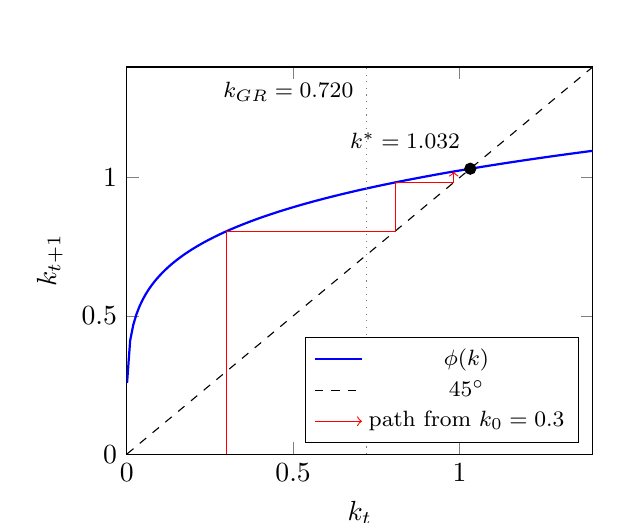
\begin{tikzpicture}\begin{axis}[width=7.5cm,height=6.5cm,xmin=0,xmax=1.4,ymin=0,ymax=1.4,xlabel={$k_t$},ylabel={$k_{t+1}$},
legend pos=south east,legend style={font=\footnotesize},samples=150,domain=0.001:1.4]
\addplot[blue,thick] {1.0256*x^(0.2)};
\addplot[black,dashed] {x};
\addplot[red,thin,->] coordinates {(0.3,0) (0.3,0.8062) (0.8062,0.8062) (0.8062,0.9824) (0.9824,0.9824) (0.9824,1.0220)};
\addplot[only marks,mark=*] coordinates {(1.0322,1.0322)};
\addplot[gray,dotted] coordinates {(0.7204,0) (0.7204,1.4)};
\legend{$\phi(k)$, $45^\circ$, path from $k_0=0.3$}
\node[anchor=north east,font=\footnotesize] at (axis cs:0.71,1.38) {$k_{GR}=0.720$};
\node[anchor=south east,font=\footnotesize] at (axis cs:1.03,1.07) {$k^\ast=1.032$};
\end{axis}\end{tikzpicture}\end{center}
Solow's discrete law with $\delta=1$ is
\begin{equation}
k_{t+1}=\frac{s_SAk_t^\alpha}{1+n}. \label{q10:solow}
\end{equation}
\eqref{q10:lom1} is \eqref{q10:solow} with $s_S=\frac{(1-\alpha)\beta}{1+\beta}$; with $\sigma\ne1$, \eqref{q10:lom} shows that the rate
$s_S=(1-\alpha)s(r_{t+1})$ moves along the transition, so Solow's constant $s$ holds only in the log case.
\intuicao{$r<n$ says capital earns less than the economy's growth rate: a chain of transfers from young to old would beat saving.
Whether the market gets there depends on how saving responds to $r$, which is $\sigma$.}
\refbib{Kurlat (2020), \S6.2 and Exercise 6.1(e) (sign of $\partial c_1/\partial r$); \S4.3 (golden rule with $n$). Romer (2012), \S\S2.9--2.10, eqs.\ (2.55)--(2.60),
pp.~78--88, and \S2.11 (dynamic inefficiency), pp.~88--91; Romer, \emph{Solution Manual}, Problem 2.16(b) for the log case.}
\rubrica{
\item (a) $s(r)$ and the sign of $s'$ with its reading: 3 pts; sign read as $\sigma-1$: max.\ 1 pt.
\item (b): 3 pts; no market clearing: 0 for (b). (c): 3 pts; identity $I/Y=\alpha(1+n)/(1+r)$ quoted: max.\ 1 pt.
\item (d): 2 pts. (e) diagram (axes, $45^\circ$, curve, $k^\ast$, $k_{GR}$) and the Solow reading: 2 pts.
}
\end{sol}


\end{document}
